\documentclass[english,11pt]{beamer}

\DeclareMathOperator{\Cov}{Cov}
\DeclareMathOperator{\Var}{Var}
\DeclareMathOperator{\E}{\mathbb{E}}
\DeclareMathOperator{\Proba}{\mathbb{P}}

\newcommand{\Covb}[2]{\ensuremath{\Cov\!\left[#1,#2\right]}}
\newcommand{\Eb}[1]{\ensuremath{\E\!\left[#1\right]}}
\newcommand{\Pb}[1]{\ensuremath{\Proba\!\left[#1\right]}}
\newcommand{\Varb}[1]{\ensuremath{\Var\!\left[#1\right]}}

% norm
\newcommand{\norm}[1]{\| #1 \|}

\newcommand{\indep}{\rotatebox[origin=c]{90}{$\models$}}





\usepackage{mathptmx,amsmath,amssymb,graphicx,bibentry,bbm,babel,ragged2e}

\makeatletter

\newcommand{\noun}[1]{\textsc{#1}}
\newcommand{\jitem}[1]{\item \begin{justify} #1 \end{justify} \vfill{}}
\newcommand{\sframe}[2]{\frame{\frametitle{#1} #2}}

\newenvironment{centercolumns}{\begin{columns}[c]}{\end{columns}}
%\newenvironment{jitem}{\begin{justify}\begin{itemize}}{\end{itemize}\end{justify}}

\usetheme{Warsaw}
\setbeamertemplate{footline}[text line]{}
\setbeamercolor{structure}{fg=purple!50!blue, bg=purple!50!blue}

\setbeamersize{text margin left=15pt,text margin right=15pt}

\setbeamercovered{transparent}


\@ifundefined{showcaptionsetup}{}{%
 \PassOptionsToPackage{caption=false}{subfig}}
\usepackage{subfig}

\usepackage[utf8]{inputenc}
\usepackage[T1]{fontenc}

\usepackage{multirow}


\makeatother

\begin{document}





\title{Multi-modeling the morphogenesis of transportation networks}

\author{J.~Raimbault$^{1,2,\ast}$\\
\texttt{juste.raimbault@iscpif.fr}
}


\institute{$^{1}$Complex Systems Institute, Paris, UPS CNRS 3611 ISC-PIF\\
$^{2}$UMR CNRS 8504 G{\'e}ographie-cit{\'e}s
}


\date{ALife 2018\\\smallskip
Tokyo\\\smallskip
July 26th 2018
}

\frame{\maketitle}


% This research introduces a multi-modeling approach to the growth of transportation networks. More precisely, we implement and compare several models, based on biological net- work growth, cost-benefit rules, and gravity potential break- down. The resulting multi-modeling framework is calibrated on observed topological data for the European road network. We show that different heuristics are complementary to cover the feasible topological space and that all are necessary to approach existing configurations, what suggests the superposition of corresponding processes in territorial systems.



%%%%%%%%%%%%%%%%%
%\section{Introduction}
%%%%%%%%%%%%%%%%%




\sframe{Urban growth and network growth}{

\centering

\begin{columns}

\begin{column}{0.42\textwidth}
	\frame{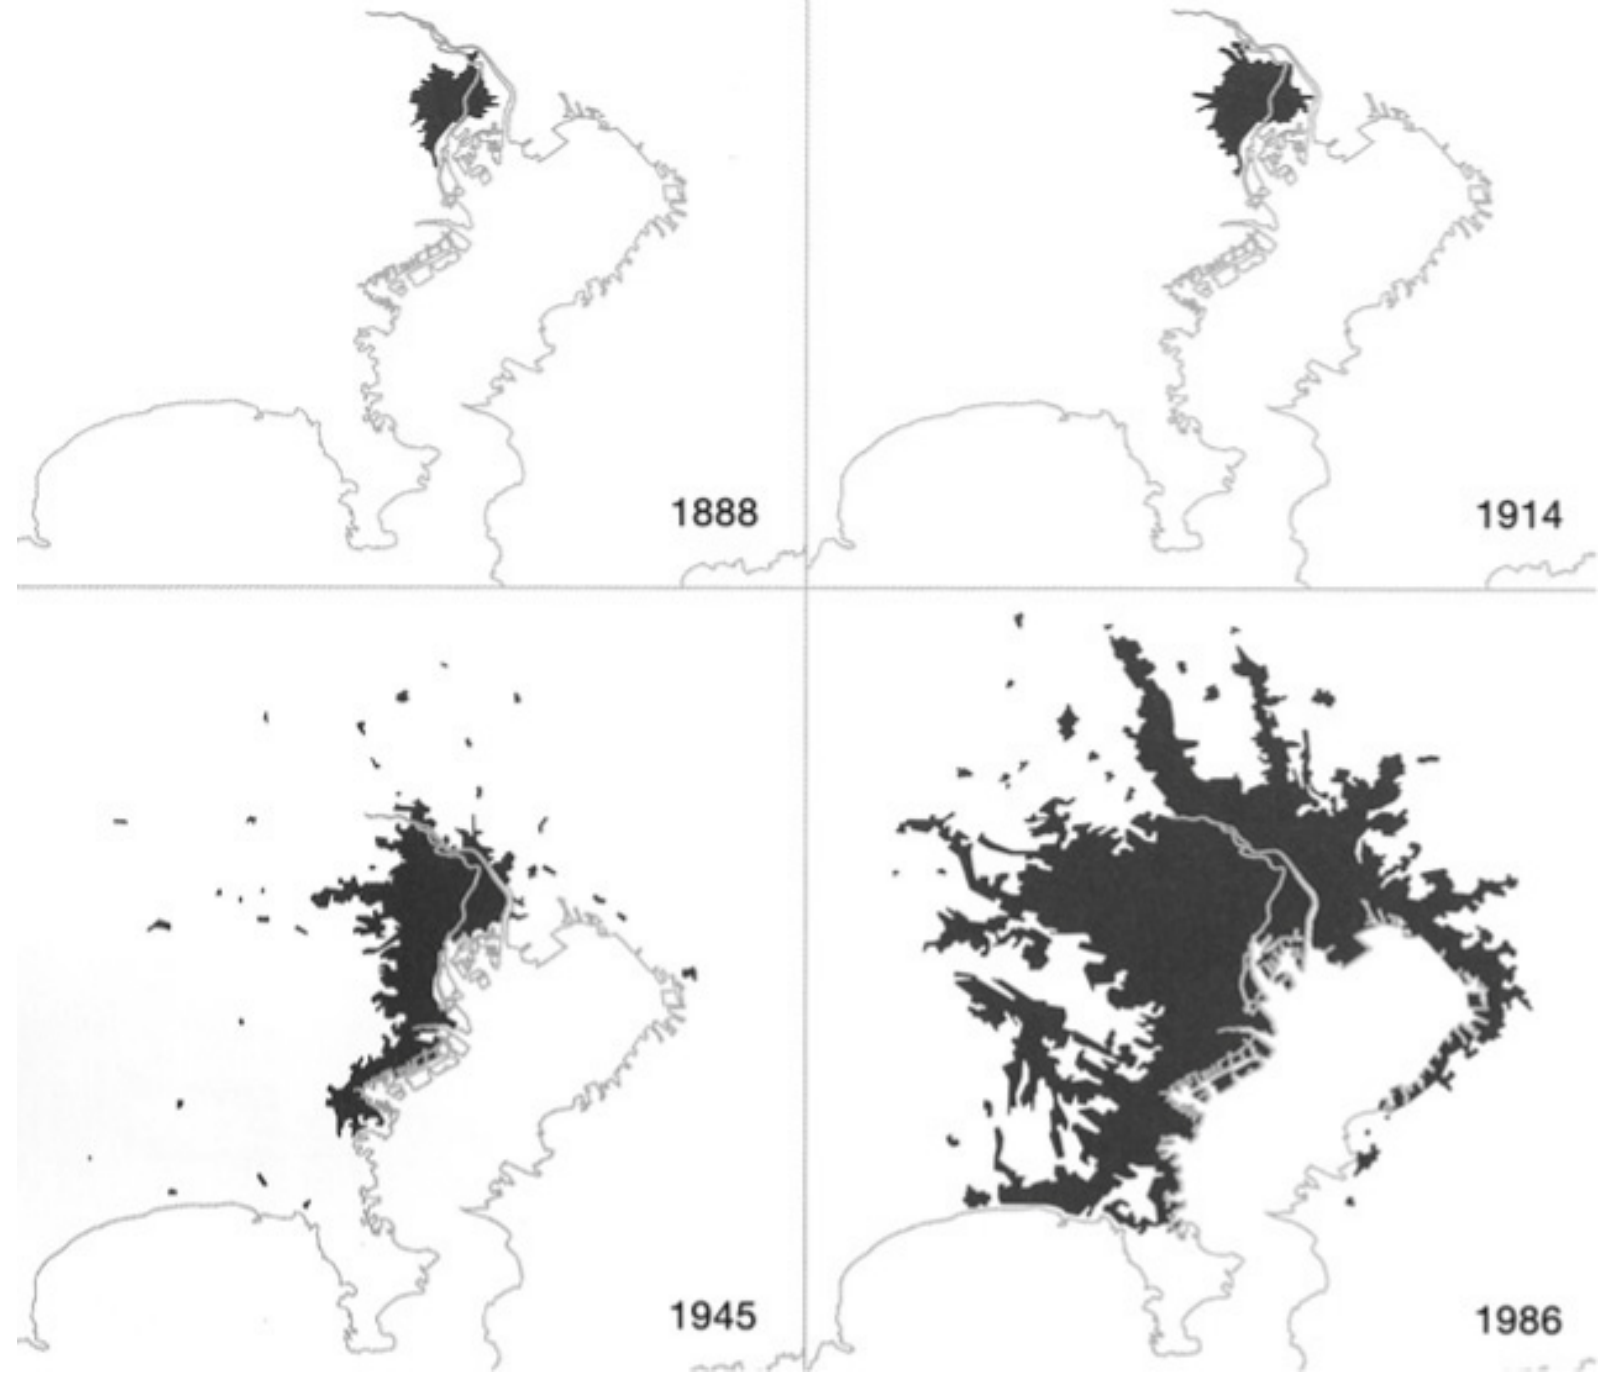
\includegraphics[width=\textwidth,height=0.4\textheight]{figures/intro_dongjingdensity.png}}\\
	\frame{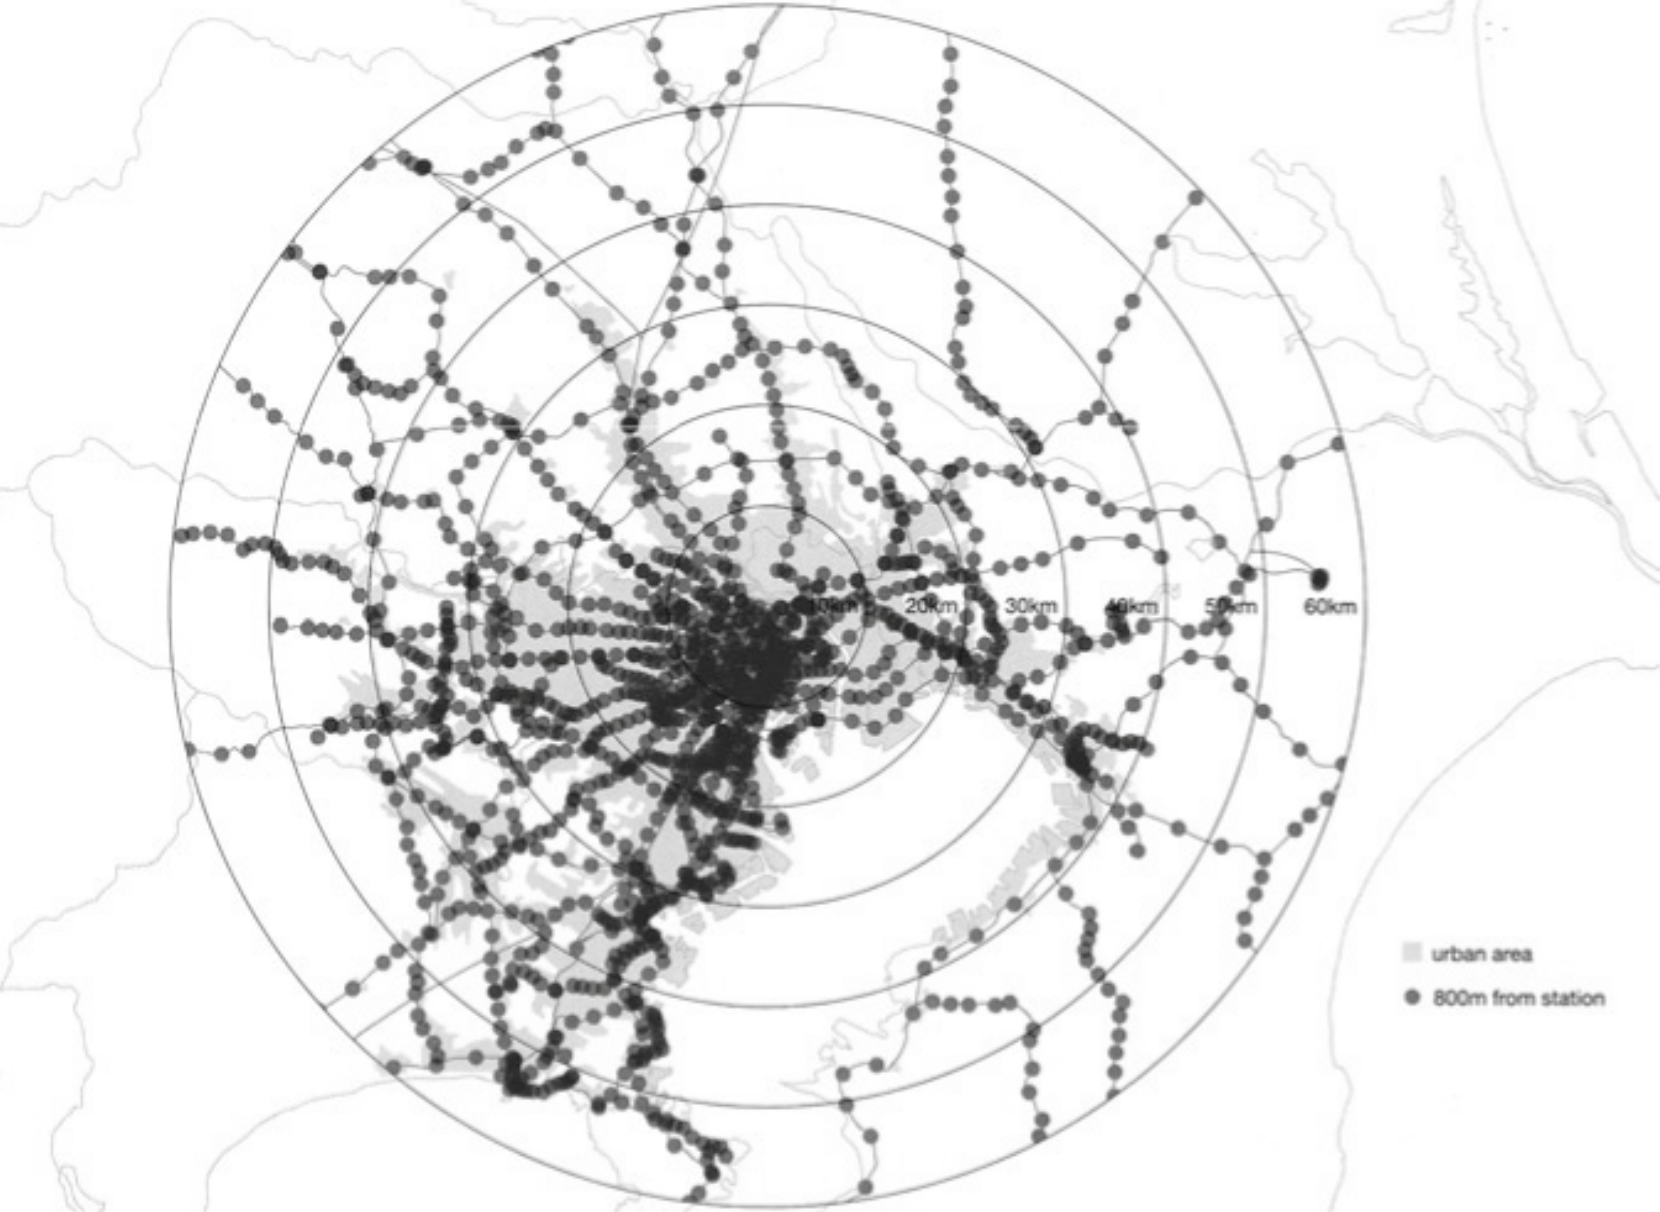
\includegraphics[width=\textwidth,height=0.4\textheight]{figures/intro_dongjingditie.png}}
\footnotesize
\textit{Source: \cite{okata2011tokyo}}

\end{column}

\begin{column}{0.5\textwidth}
	
	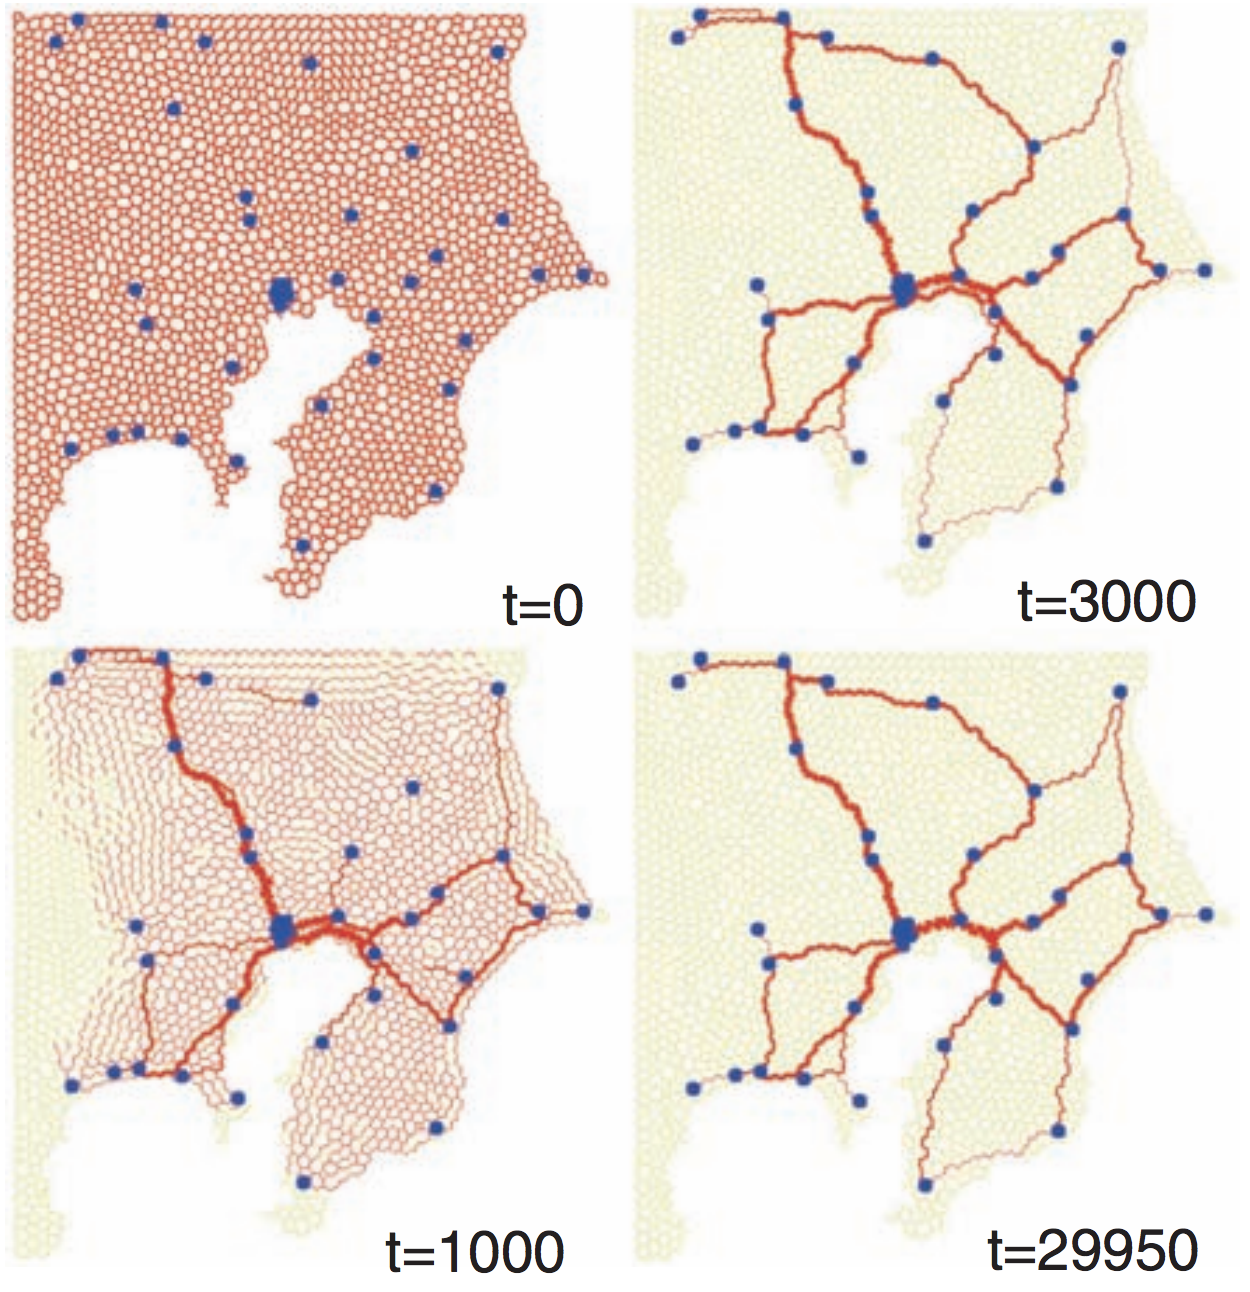
\includegraphics[width=\textwidth]{figures/intro_tero.png}
	
	\footnotesize
\textit{Source: \cite{tero2010rules}}

	
\end{column}


\end{columns}


}


\sframe{Transportation networks}{

\centering

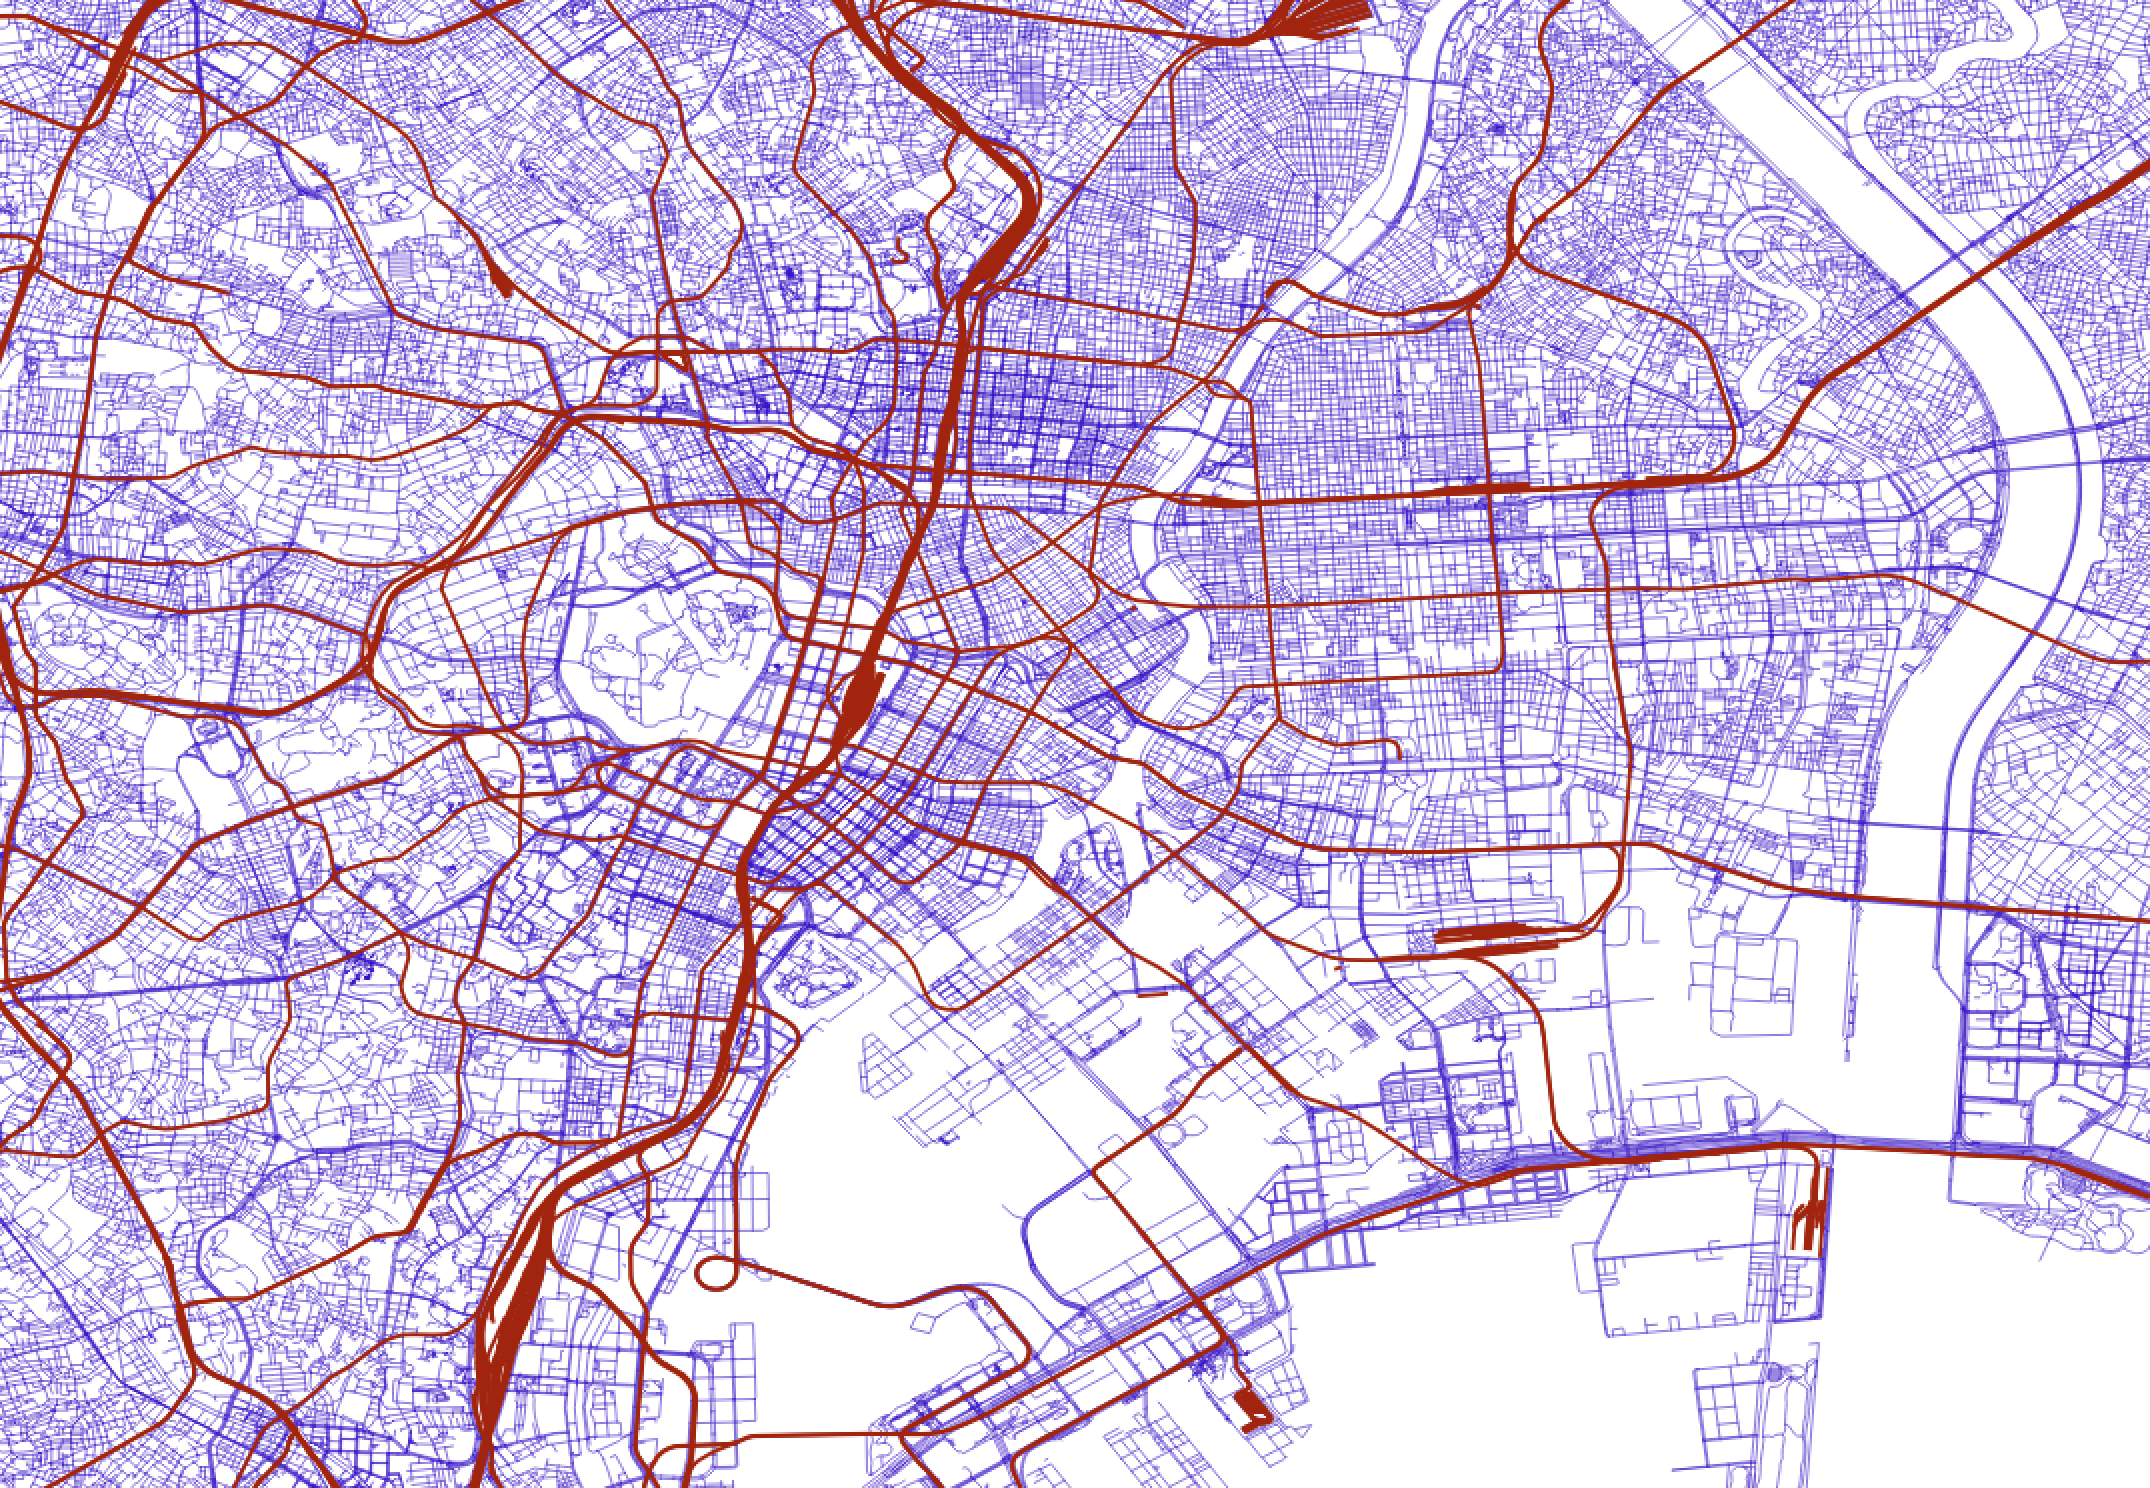
\includegraphics[width=0.95\textwidth]{figures/intro_tokyoosm.png}

\footnotesize \textit{Source: OpenStreetMap}

}


\sframe{Morphogenesis of transportation networks}{

\justify

\vspace{-0.5cm}

\textit{Is the city alive ? } \textbf{No}

\medskip

\textit{Is the city ALife ? } \textbf{Kind of}

\medskip

%\normalsize

$\rightarrow$ Cities (territorial systems) are morphogenetic \cite{doursat2012morphogenetic}

% The growth of transportation networks in territorial sys- tems bears stunning similarities with biological networks, and the understanding of processes driving their spatial ex- tension can both have practical planning applications but also bring theoretical insights into complex morphogenetic systems. Network growth models have been proposed in several disciplines, of which Xie and Levinson (2009) give a large overview, taking into account diverse processes such as economical, geometrical, geographical processes for ex- ample. There exists to our knowledge no systematic compar- ison of different network generation heuristics. We develop here such a comparison in a multi-modeling paradigm.

%\vspace{1.5cm}

\medskip

\centering

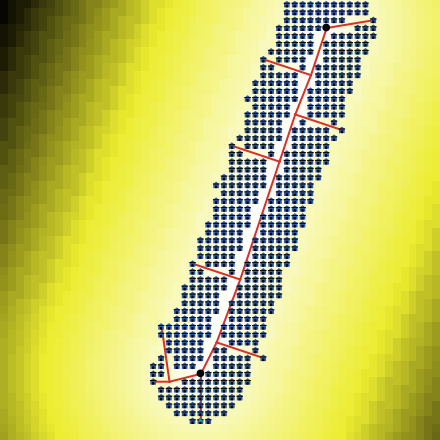
\includegraphics[width=0.3\textwidth]{figures/rbd_corbuLinearCiudad.png}\hspace{0.1cm}
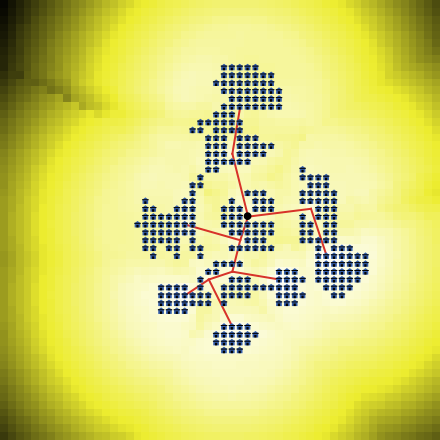
\includegraphics[width=0.3\textwidth]{figures/rbd_corbuRadiant.png}\hspace{0.1cm}
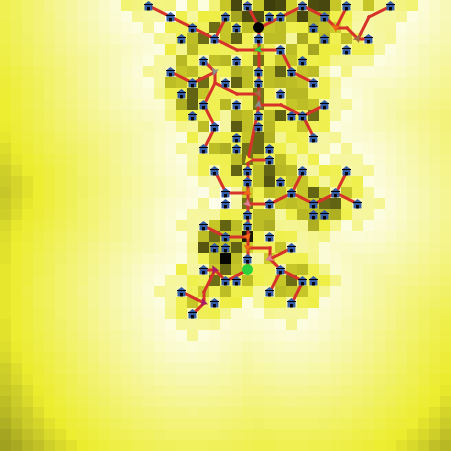
\includegraphics[width=0.3\textwidth]{figures/rbd_TreeLikeCity.png}

\textit{Stylized urban forms \cite{raimbault2014hybrid}}

\bigskip

\raggedright

\textbf{Research objective: } \textit{Understand the morphogenesis of transportation networks (road network), taking into account multiple concurrent processes through multi-modeling}


}



% Modeling network growth
% We introduce a general model of road network growth, con- ditioned to a fixed population density on a grid, in a se- quential way with the following steps. A common core en- sures the positioning of new centers preferentially to pop- ulation density and a direct connection to the existing net- work. Nodes and links are then added following different potential processes corresponding to the selected heuristic: (i) no supplementary growth (baseline); (ii) random links; (iii) biological network growth following the model of Tero et al. (2010), where new links are taken as the links with the highest capacity in the stationary flow network obtained by evolving capacities of the full network of potential new links; (iv) cost-benefit network growth as proposed by Louf et al. (2013); (v) stochastic gravity potential breakdown as used by Schmitt (2014); and (vi) a novel model based on thresholded deterministic potential breakdown. The network is grown until reaching a fixed number of new nodes to en- sure comparability between the different heuristics.

% model description




\sframe{Road network generation algorithm}{

At each time step, with a fixed population density: 

\begin{enumerate}
	\item Add new nodes preferentially to population and connect them
	\item \justify Variable heuristic for new links, among: nothing, random, gravity-based deterministic breakdown, gravity-based random breakdown (from \cite{schmitt2014modelisation}), cost-benefits (from \cite{louf2013emergence}), biological network generation (based on \cite{tero2010rules})
\end{enumerate}

\medskip

\centering

\frame{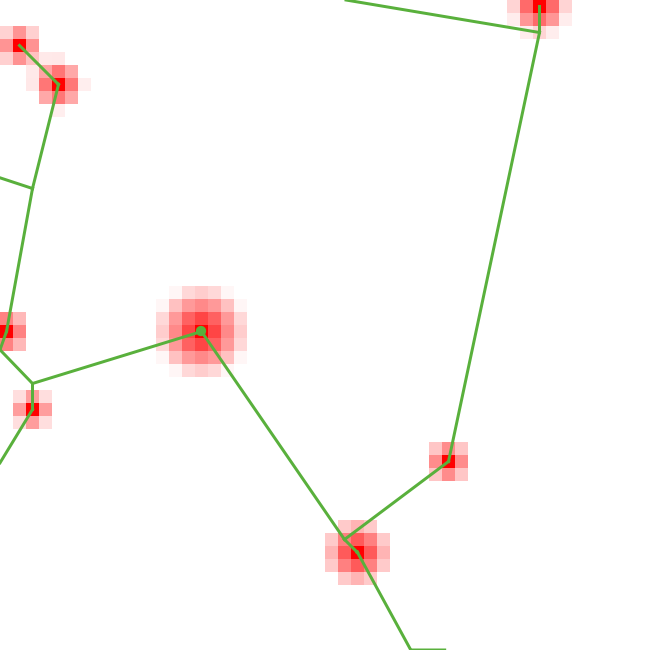
\includegraphics[width=0.32\textwidth]{figures/example_nwgrowth_tick0.png}}
\frame{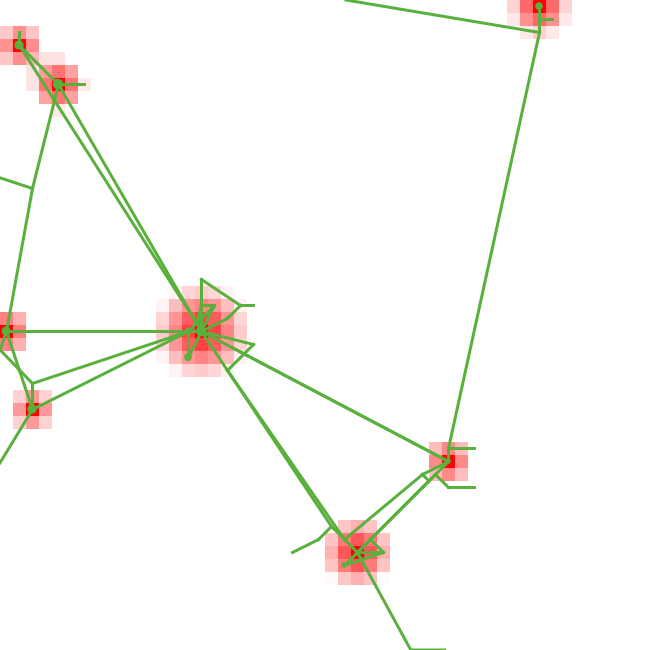
\includegraphics[width=0.32\textwidth]{figures/example_nwgrowth_tick2.png}}
\frame{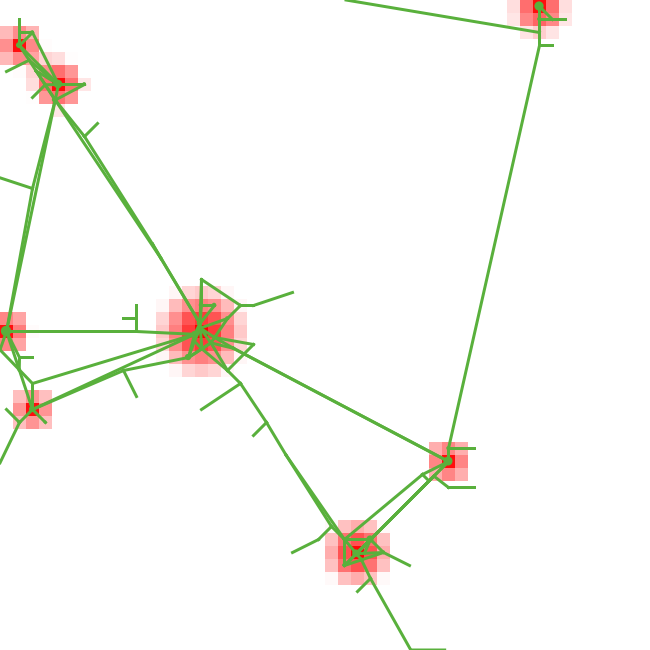
\includegraphics[width=0.32\textwidth]{figures/example_nwgrowth_tick10.png}}

}


\sframe{Biological network generation}{

Model studied by~\cite{tero2010rules} : exploration and reinforcement by a slime mould searching for ressources

\bigskip

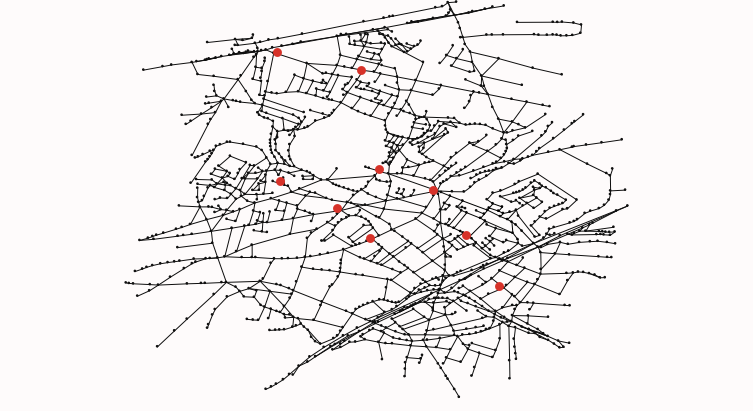
\includegraphics[width=0.32\textwidth]{figures/slimemould_tick1}
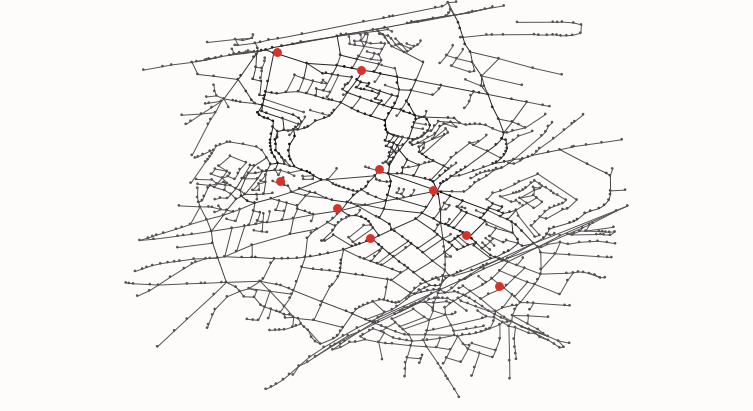
\includegraphics[width=0.32\textwidth]{figures/slimemould_tick10}
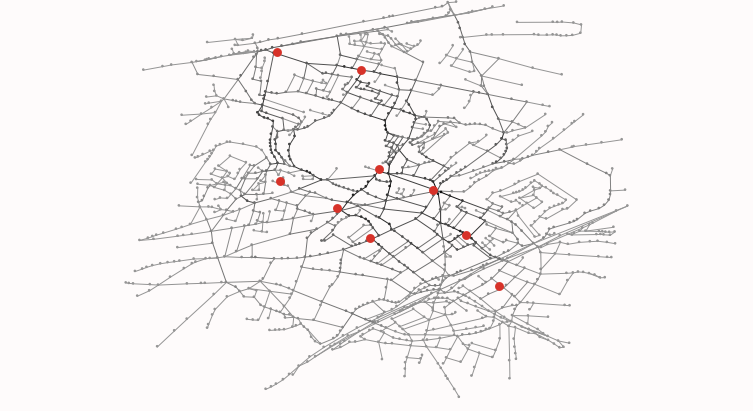
\includegraphics[width=0.32\textwidth]{figures/slimemould_tick20}\\
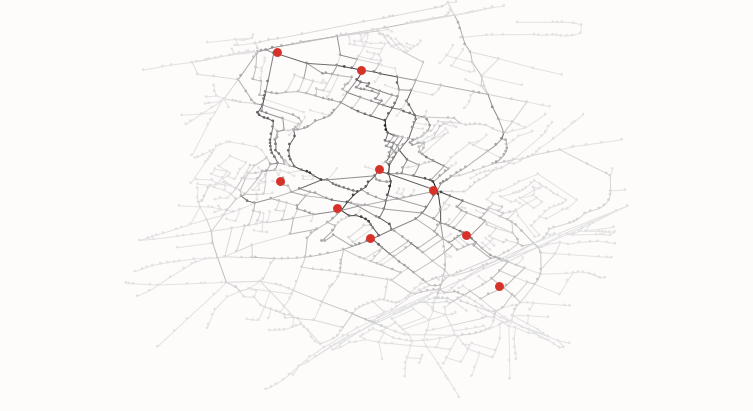
\includegraphics[width=0.32\textwidth]{figures/slimemould_tick50}
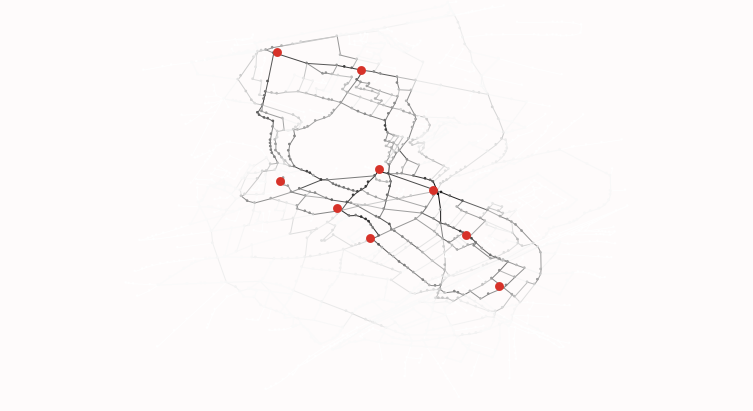
\includegraphics[width=0.32\textwidth]{figures/slimemould_tick101}
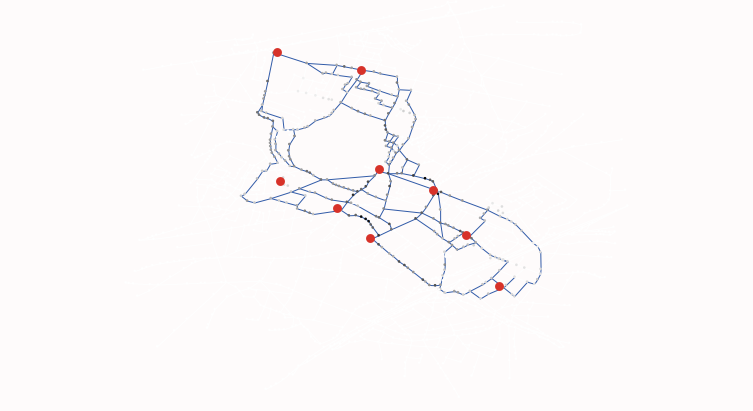
\includegraphics[width=0.32\textwidth]{figures/slimemould_reseauFinal}\\

\medskip

\footnotesize
\textit{Application to the design of optimal bus routes}

}



\sframe{Application: generating synthetic networks}{

\centering

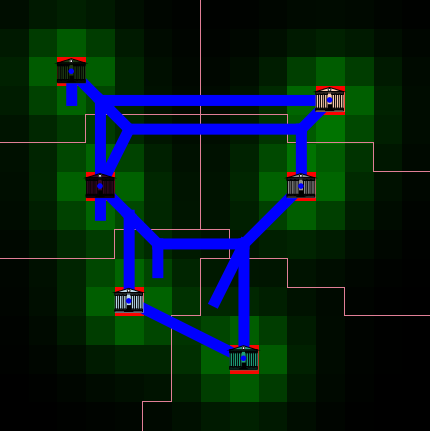
\includegraphics[width=0.32\textwidth]{figures/bionw_territ6_gamma1_1_bis.png}
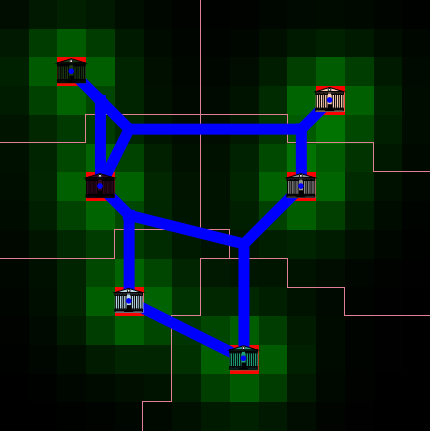
\includegraphics[width=0.32\textwidth]{figures/bionw_territ6_gamma1_2_quart.png}
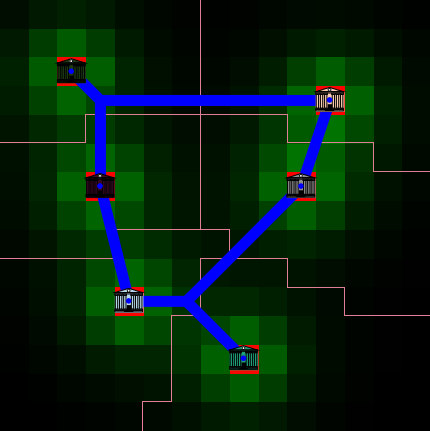
\includegraphics[width=0.32\textwidth]{figures/bionw_territ6_gamma1_3_bis.png}\\
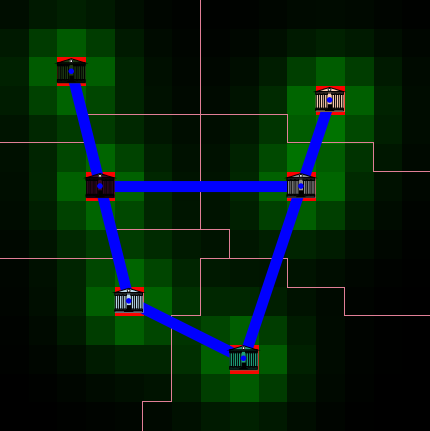
\includegraphics[width=0.32\textwidth]{figures/bionw_territ6_gamma1_5.png}
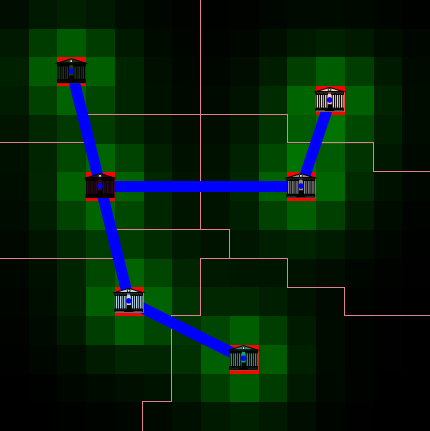
\includegraphics[width=0.32\textwidth]{figures/bionw_territ6_gamma1_8.png}
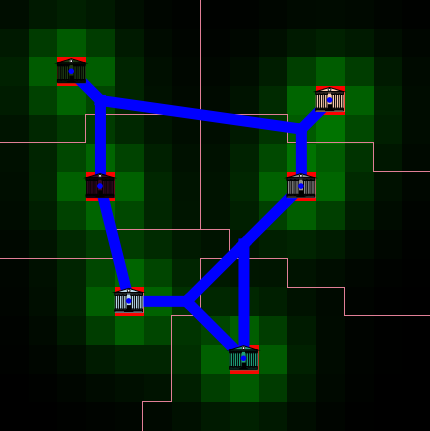
\includegraphics[width=0.32\textwidth]{figures/bionw_territ6_gamma1_25_bis.png}

\footnotesize
\textit{Generation of Pareto optimal (cost/robustness) transportation networks: transportation scenarios for a land-use model}

}

\sframe{Biological Network generation}{

Adding new links with biological heuristic:

\begin{enumerate}
	\item Create network of potential new links, with existing network and randomly sampled diagonal lattice
	\item Iterate for $k$ increasing ($k\in \{ 1,2,4 \}$ in practice) :
	\begin{itemize}
		\item Using population distribution, iterate $k\cdot n_b$ times the slime mould model to compute new link capacities
		\item Delete links with capacity under $\theta_d$
		\item Keep the largest connected component
	\end{itemize}
	\item Planarize and simplify final network
\end{enumerate}

\medskip

\centering

\frame{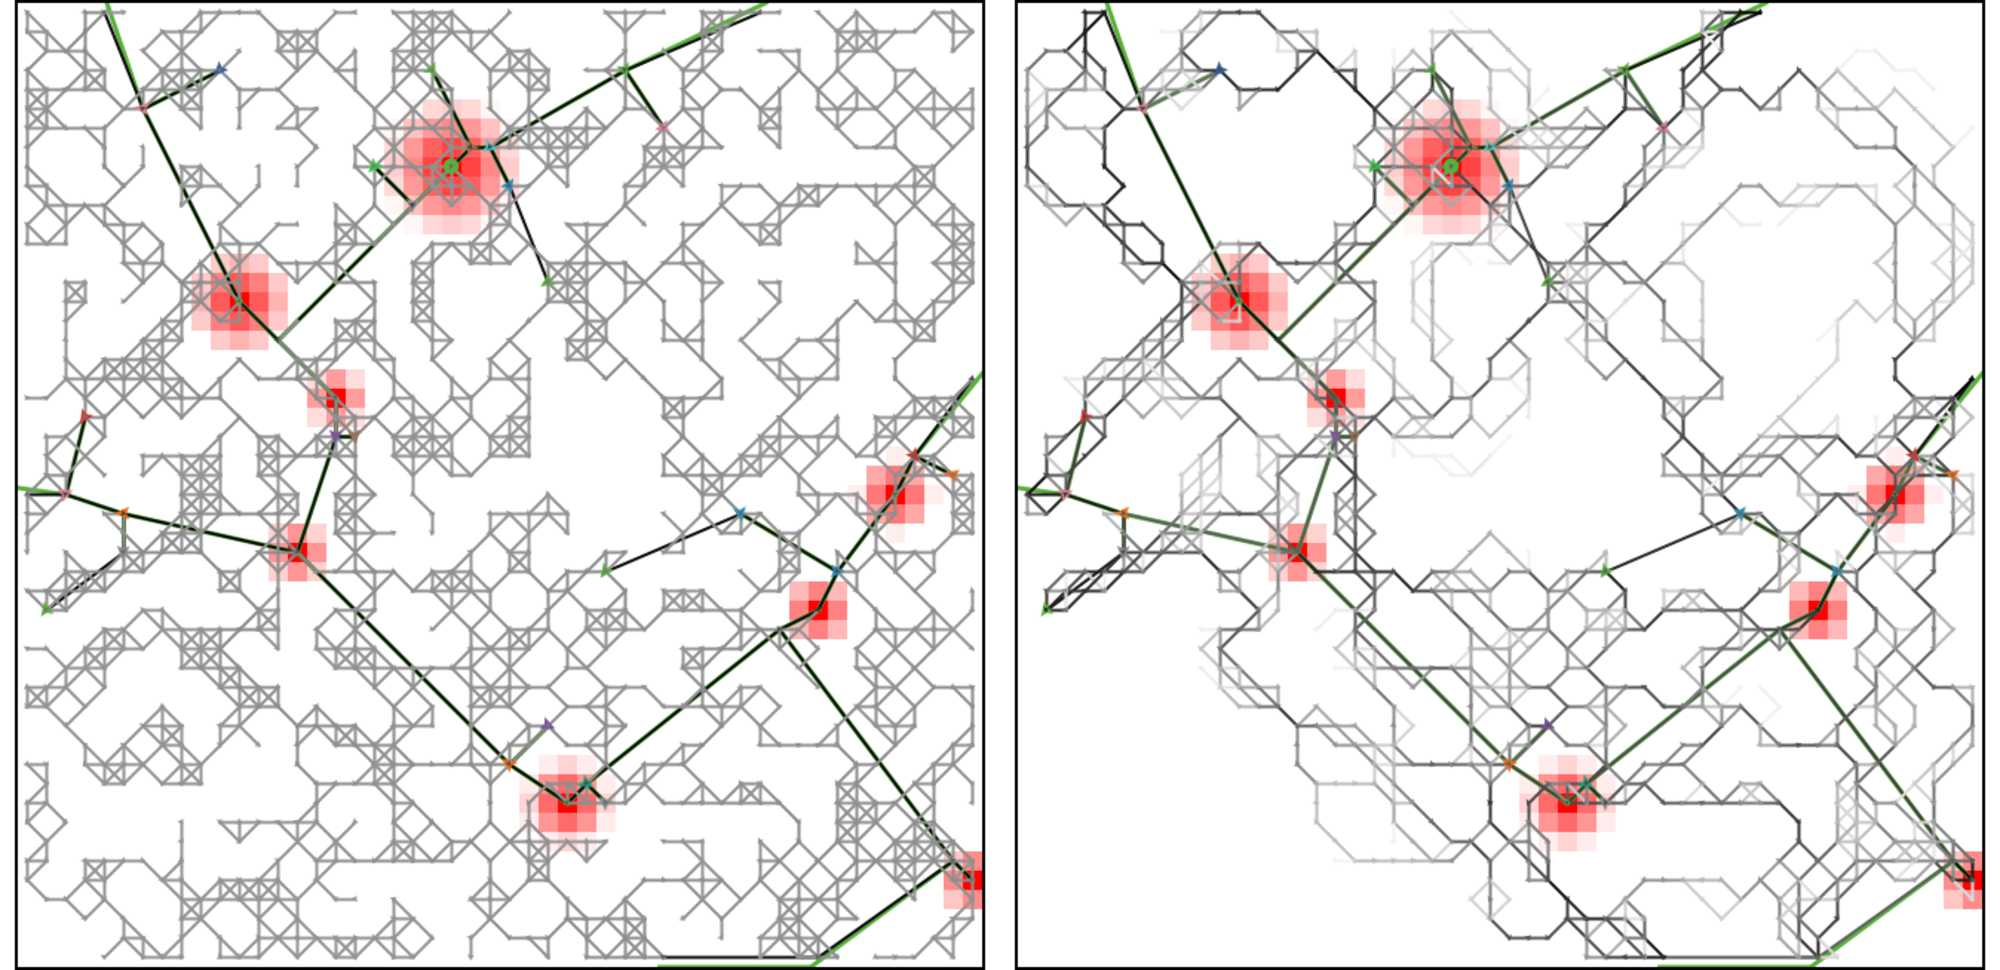
\includegraphics[width=0.6\textwidth]{figures/7-1-1-fig-networkgrowth-bioexample.jpg}}

\footnotesize

\textit{Intermediate stage for biological network generation}

}




%A network is then quantified by topological indicators, namely average closeness and betweenness centralities, di- ameter, efficiency, and average path length. To compare the generated network to real data, we collected the Euro- pean street network from the open data provided by Open- StreetMap, and extracted the value of topological indicators on 50km side moving windows. Typical configurations were then selected according to morphological classes for popu- lation density. The corresponding real network measures are compared to network generated on the same population den- sity configurations, for 50 different configurations.


\sframe{Empirical Data : network indicators}{

\centering

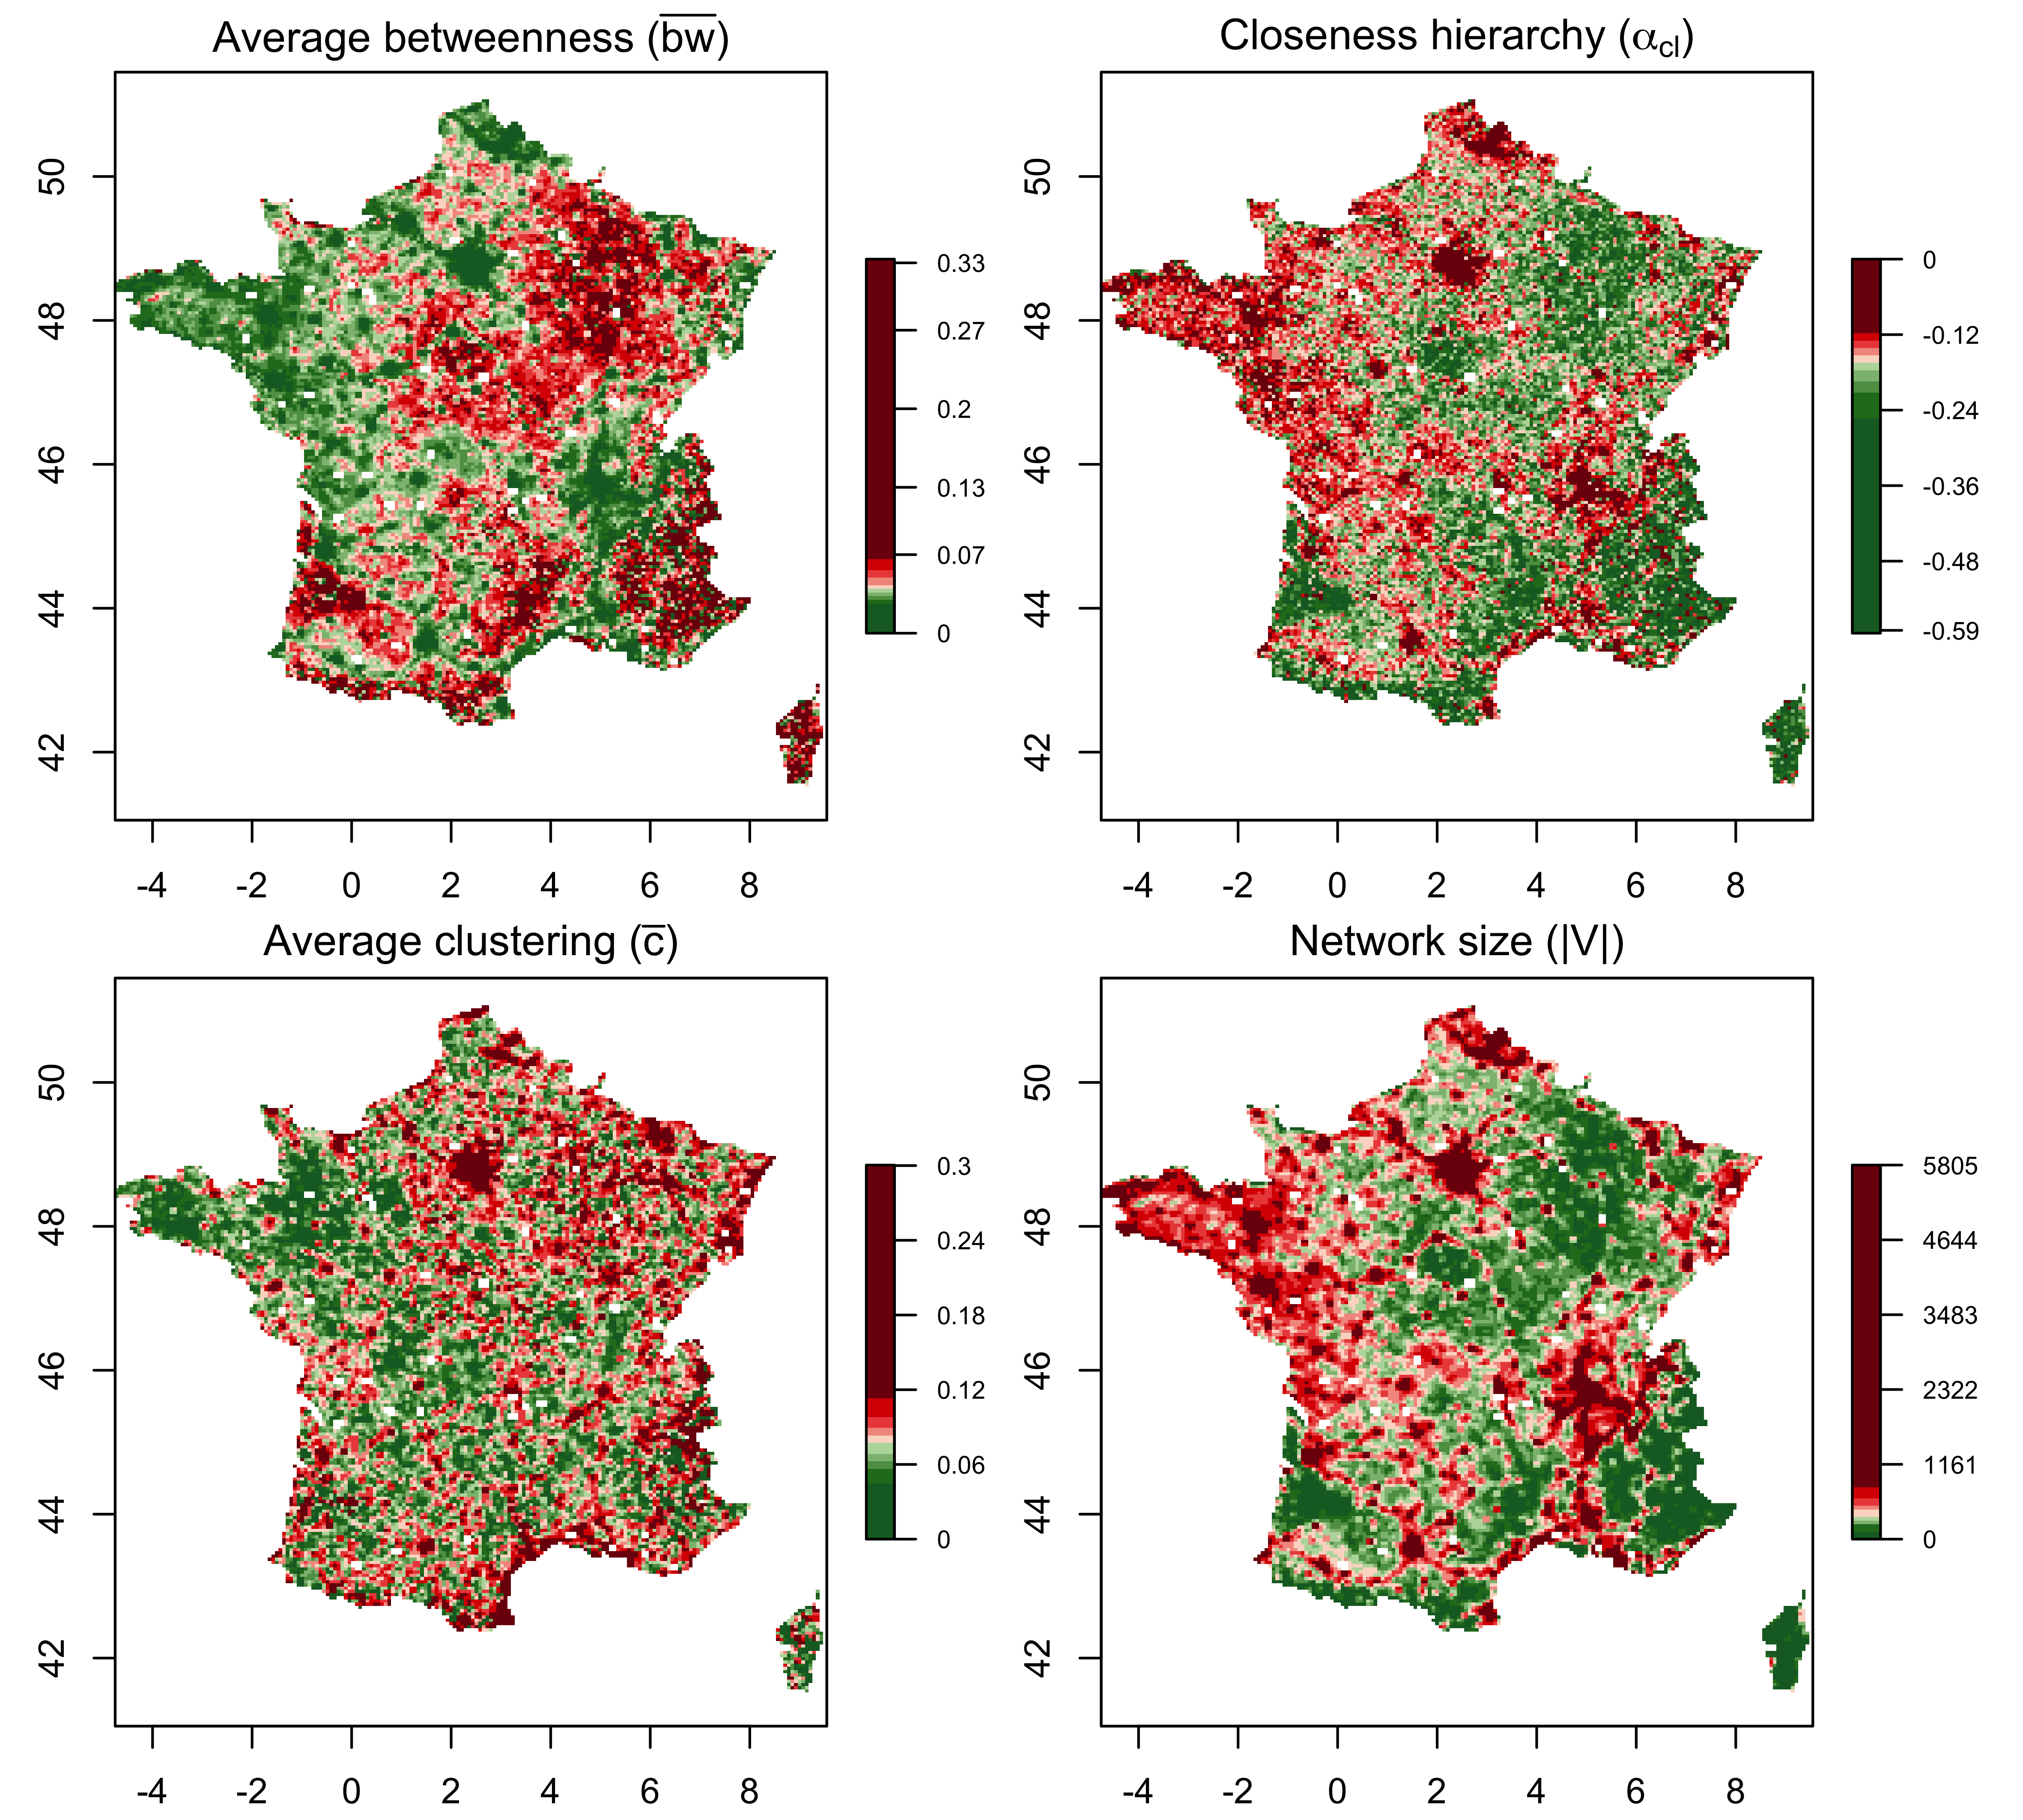
\includegraphics[width=0.8\textwidth]{figures/indics_network_en_areasize100_offset50_factor0_5.png}

}





%Results
% The heterogeneity of models suggested the choice of an im- plementation in NetLogo which handles easily heterogenous multi-agent systems. Source code and results are available on the open repository of the project1. The parameter space of the model is explored using the workflow engine Open- MOLE (Reuillon et al., 2013) which allows an easy distri- bution of tasks on a computation grid.


\sframe{Model exploration}{

Computationally intensive: high-dimensional parameter space and possible spatial setup.

\medskip

$\rightarrow$ use of grid computing, made smooth with the OpenMOLE software \url{https://next.openmole.org/}

\centering

\smallskip


\includegraphics[height=0.35\textheight]{figures/openmole.png}

\smallskip

\raggedright\justify

\footnotesize \textit{OpenMOLE: (i) embed any model as a black box; (ii) transparent access to main High Performance Computing environments; (iii) model exploration and calibration methods.}

}



% We sample for each density configuration 1000 param- eter points (including the generation heuristic and specific parameters for each heuristic in the random LHS sampling) and repeat the stochastic model 5 times for each point. Re- sults are shown in Fig. 1 below. We illustrate for a syn- thetic population density configuration the different types of networks obtained.




\sframe{Example of generated networks}{

\centering

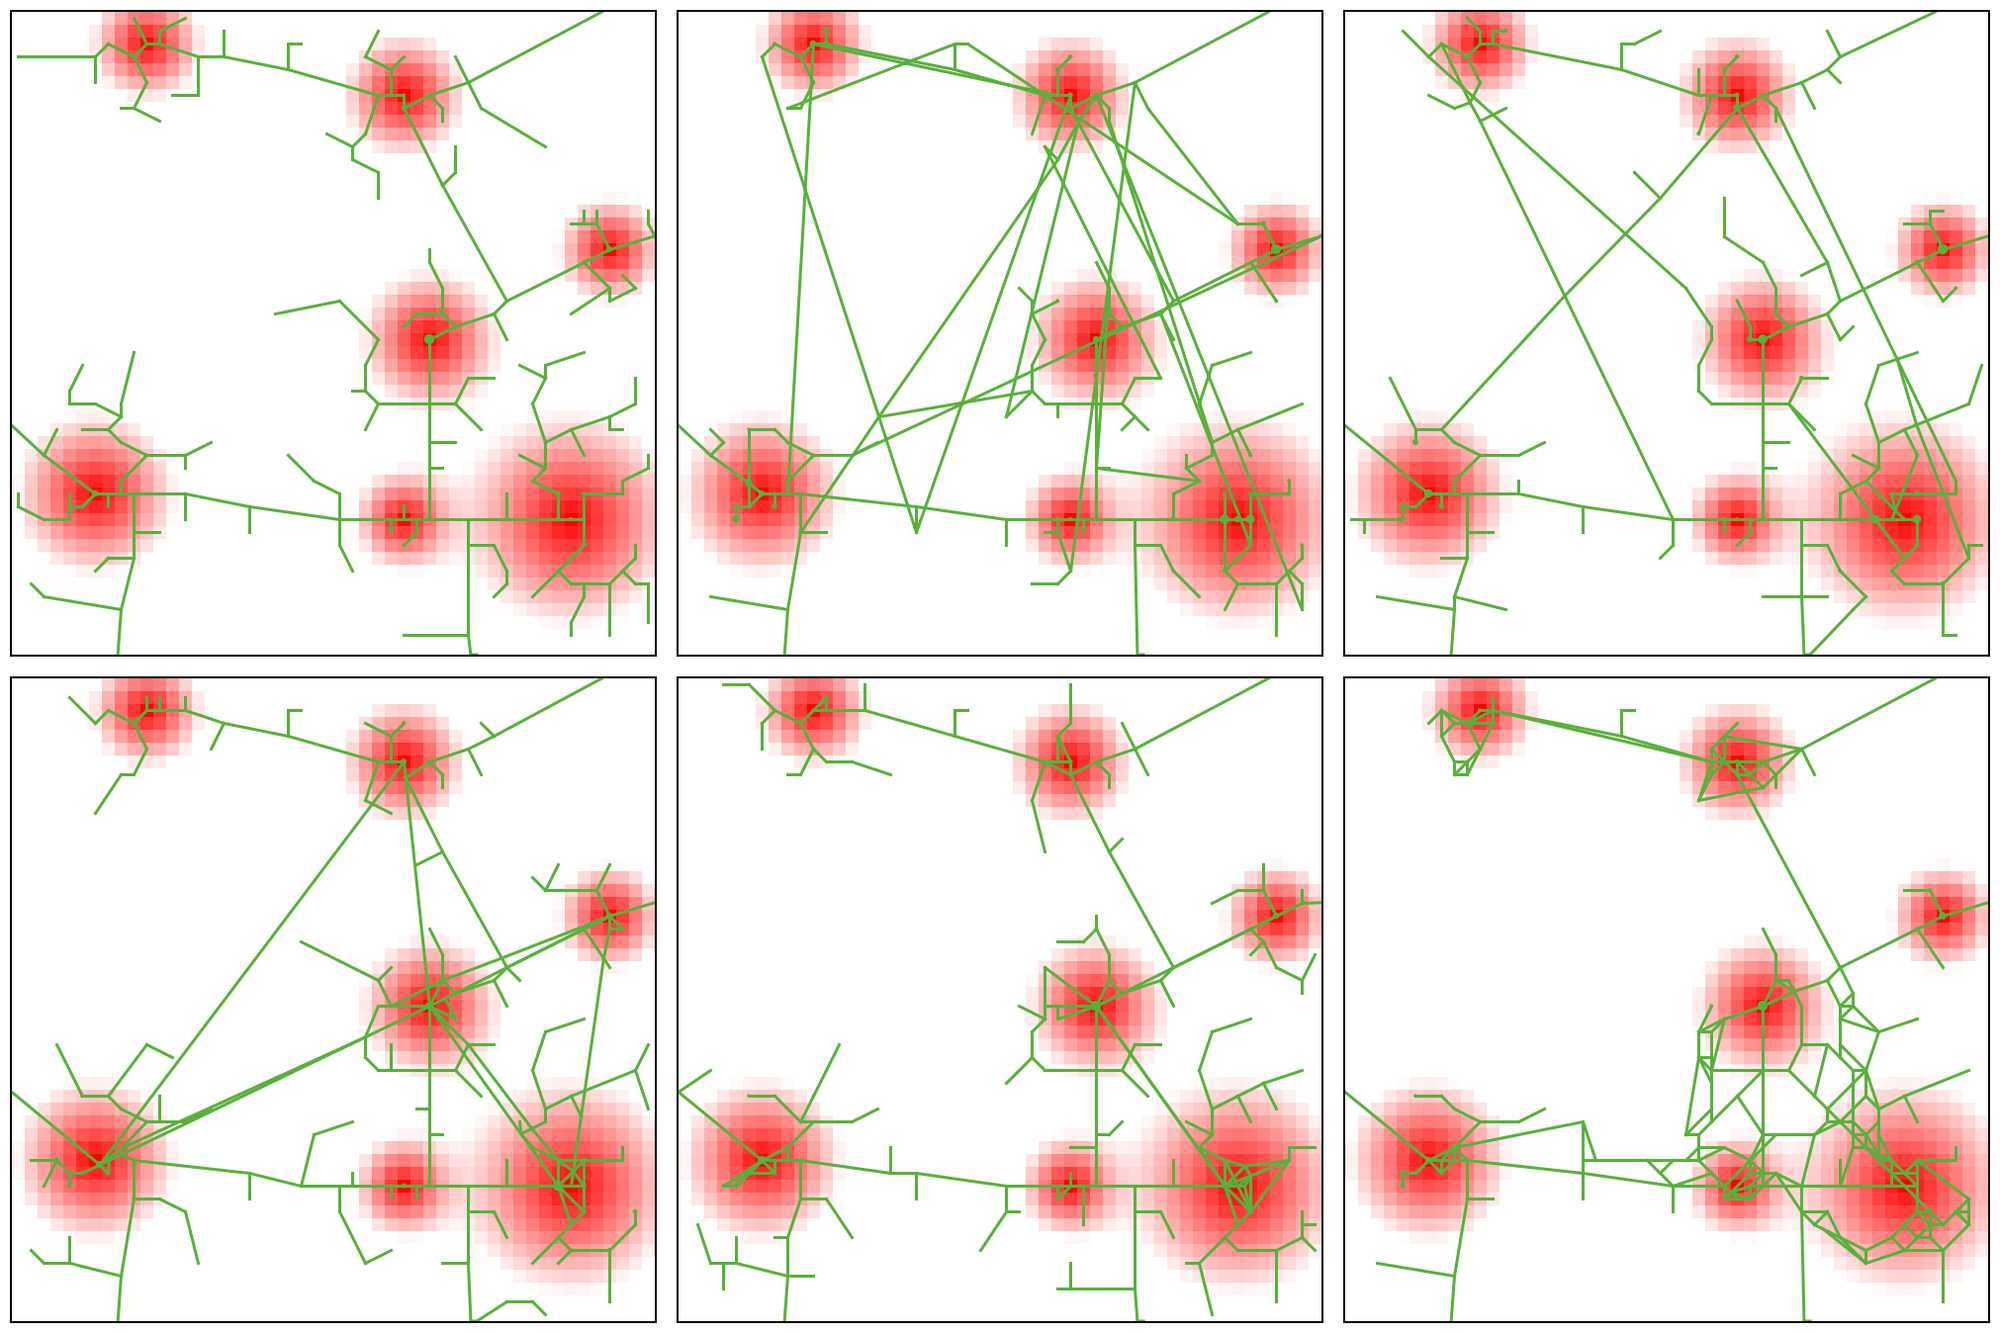
\includegraphics[width=\textwidth]{figures/7-1-2-fig-networkgrowth-examples.jpg}

\footnotesize\textit{In order: connection; random; deterministic breakdown; random breakdown; cost-driven; biological.}

}



%The feasible space covered by the sam- pling in the reduced indicator space (two first components of a principal component analysis) is such that heuristics are complementary to cover the full area, and overlap between point clouds quantified with a concentration index are low (Herfindhal index with a first quartile at 0.54 on a grid of size 20 separating the reduced indicator space). This com- plementarity is confirmed when comparing to the indicator values for real networks: some points fall relatively far from the point cloud, but each heuristic captures some real con- figurations. The distribution of distances of simulated points to real points confirm this low minimum for each heuristic. When conditioned by morphological class for population density, we obtain varying behavior regarding the most per- formant heuristic, conforming that different urban regimes are associated to specific network morphogenesis processes.



\sframe{Feasible space of network indicators}{

\centering

\hspace{-0.2cm}
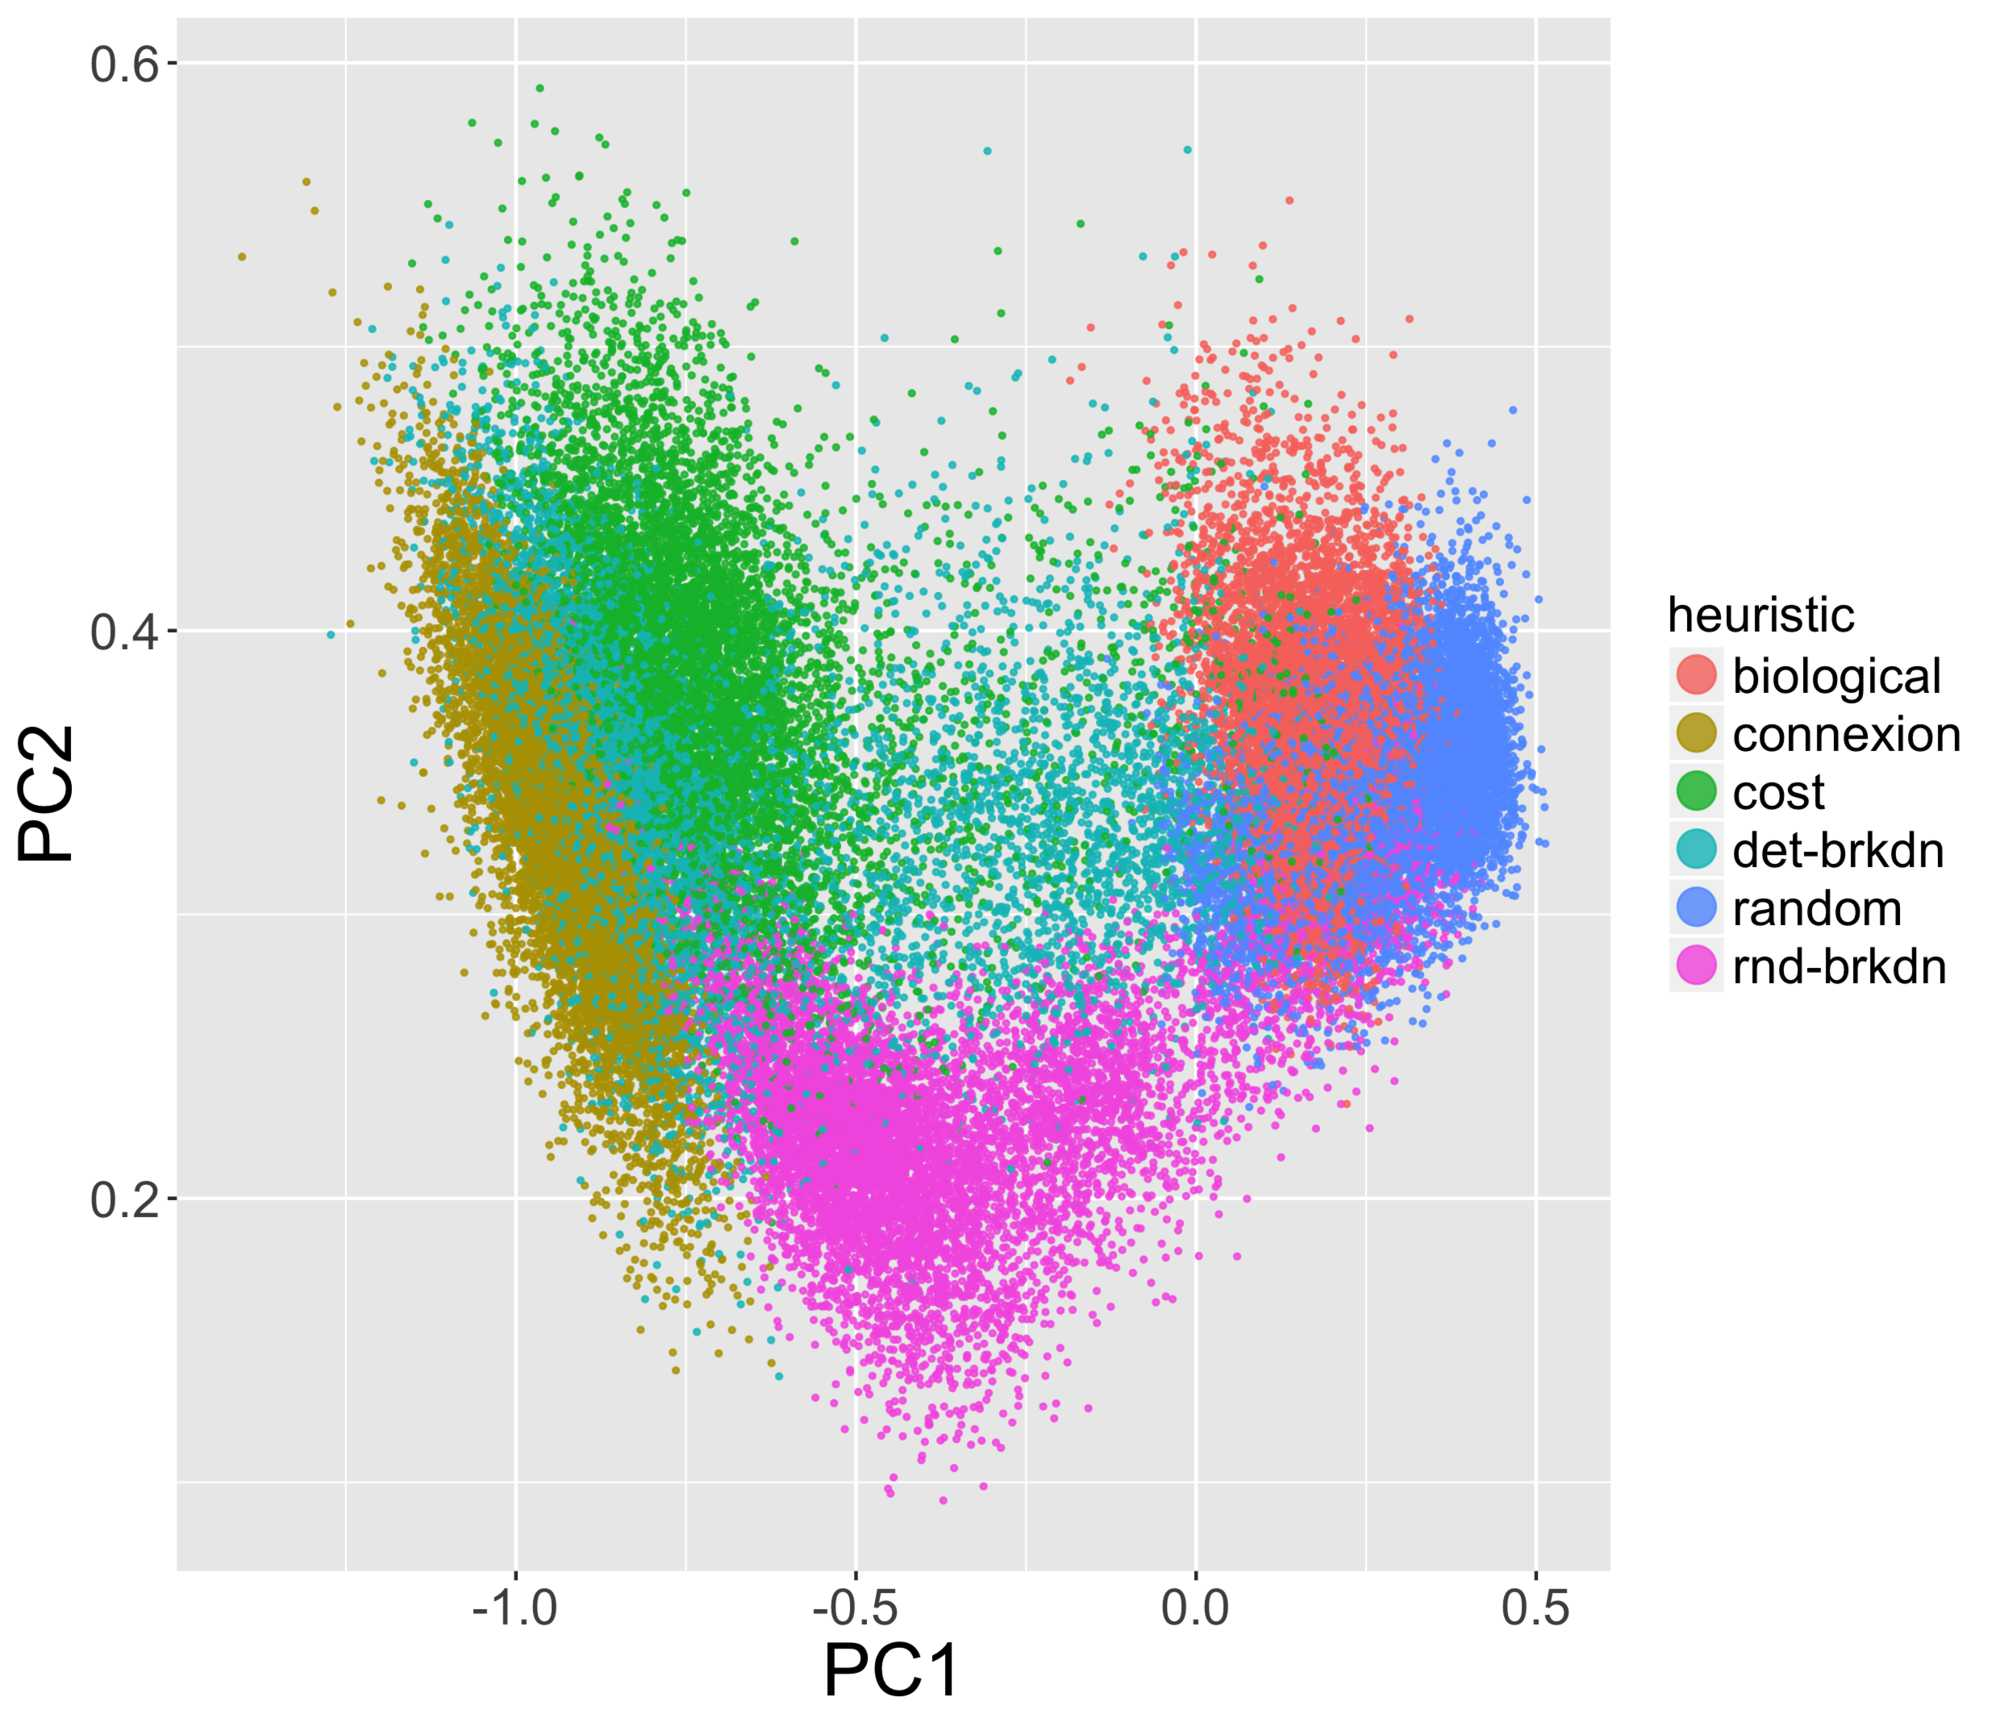
\includegraphics[width=0.53\textwidth]{figures/7-1-2-fig-networkgrowth-feasiblespace.jpg}
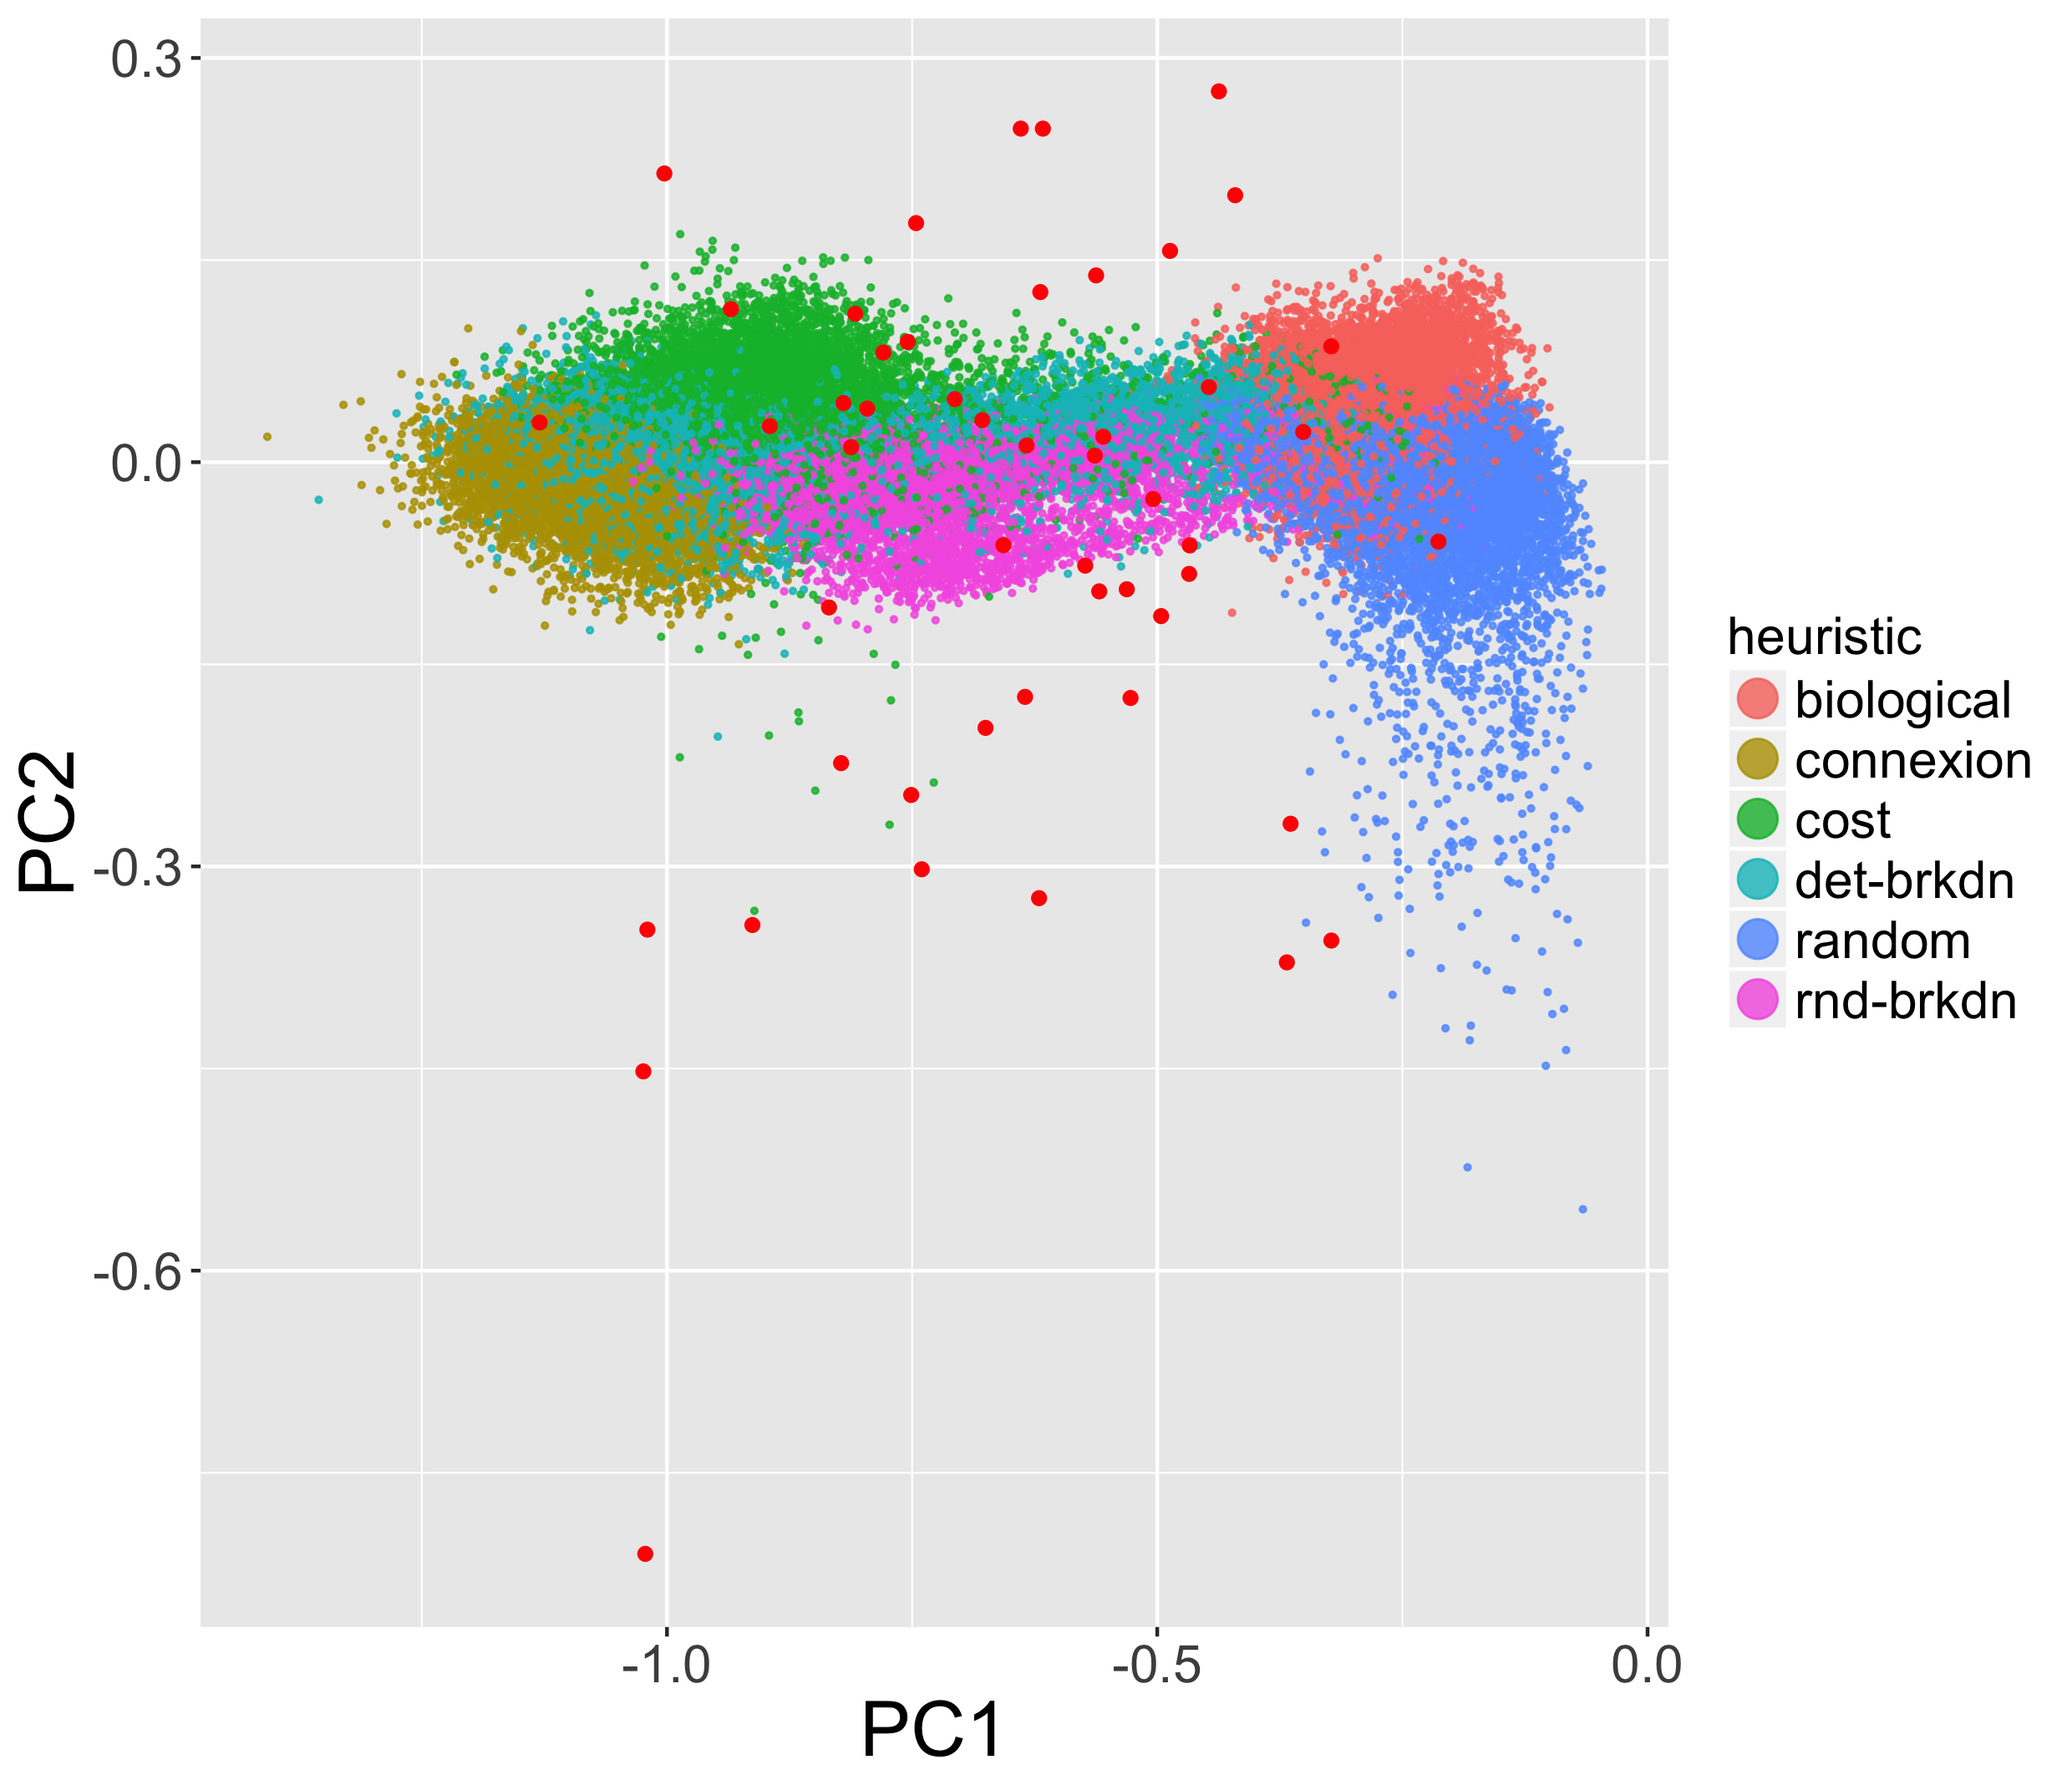
\includegraphics[width=0.53\textwidth]{figures/feasible_space_withreal_pca.png}

\raggedright\justify

\footnotesize \textit{Simulated points obtained with a LHS sampling (240000 runs, 5 repetitions for each parameter point), for real density setups (50 grids). (Left) Feasible points cloud in a reduced network indicator space; (Right) Same points with the sample of real points}

%Feasible spaces by network heuristic

}






\sframe{Distance to real networks}{

\centering

%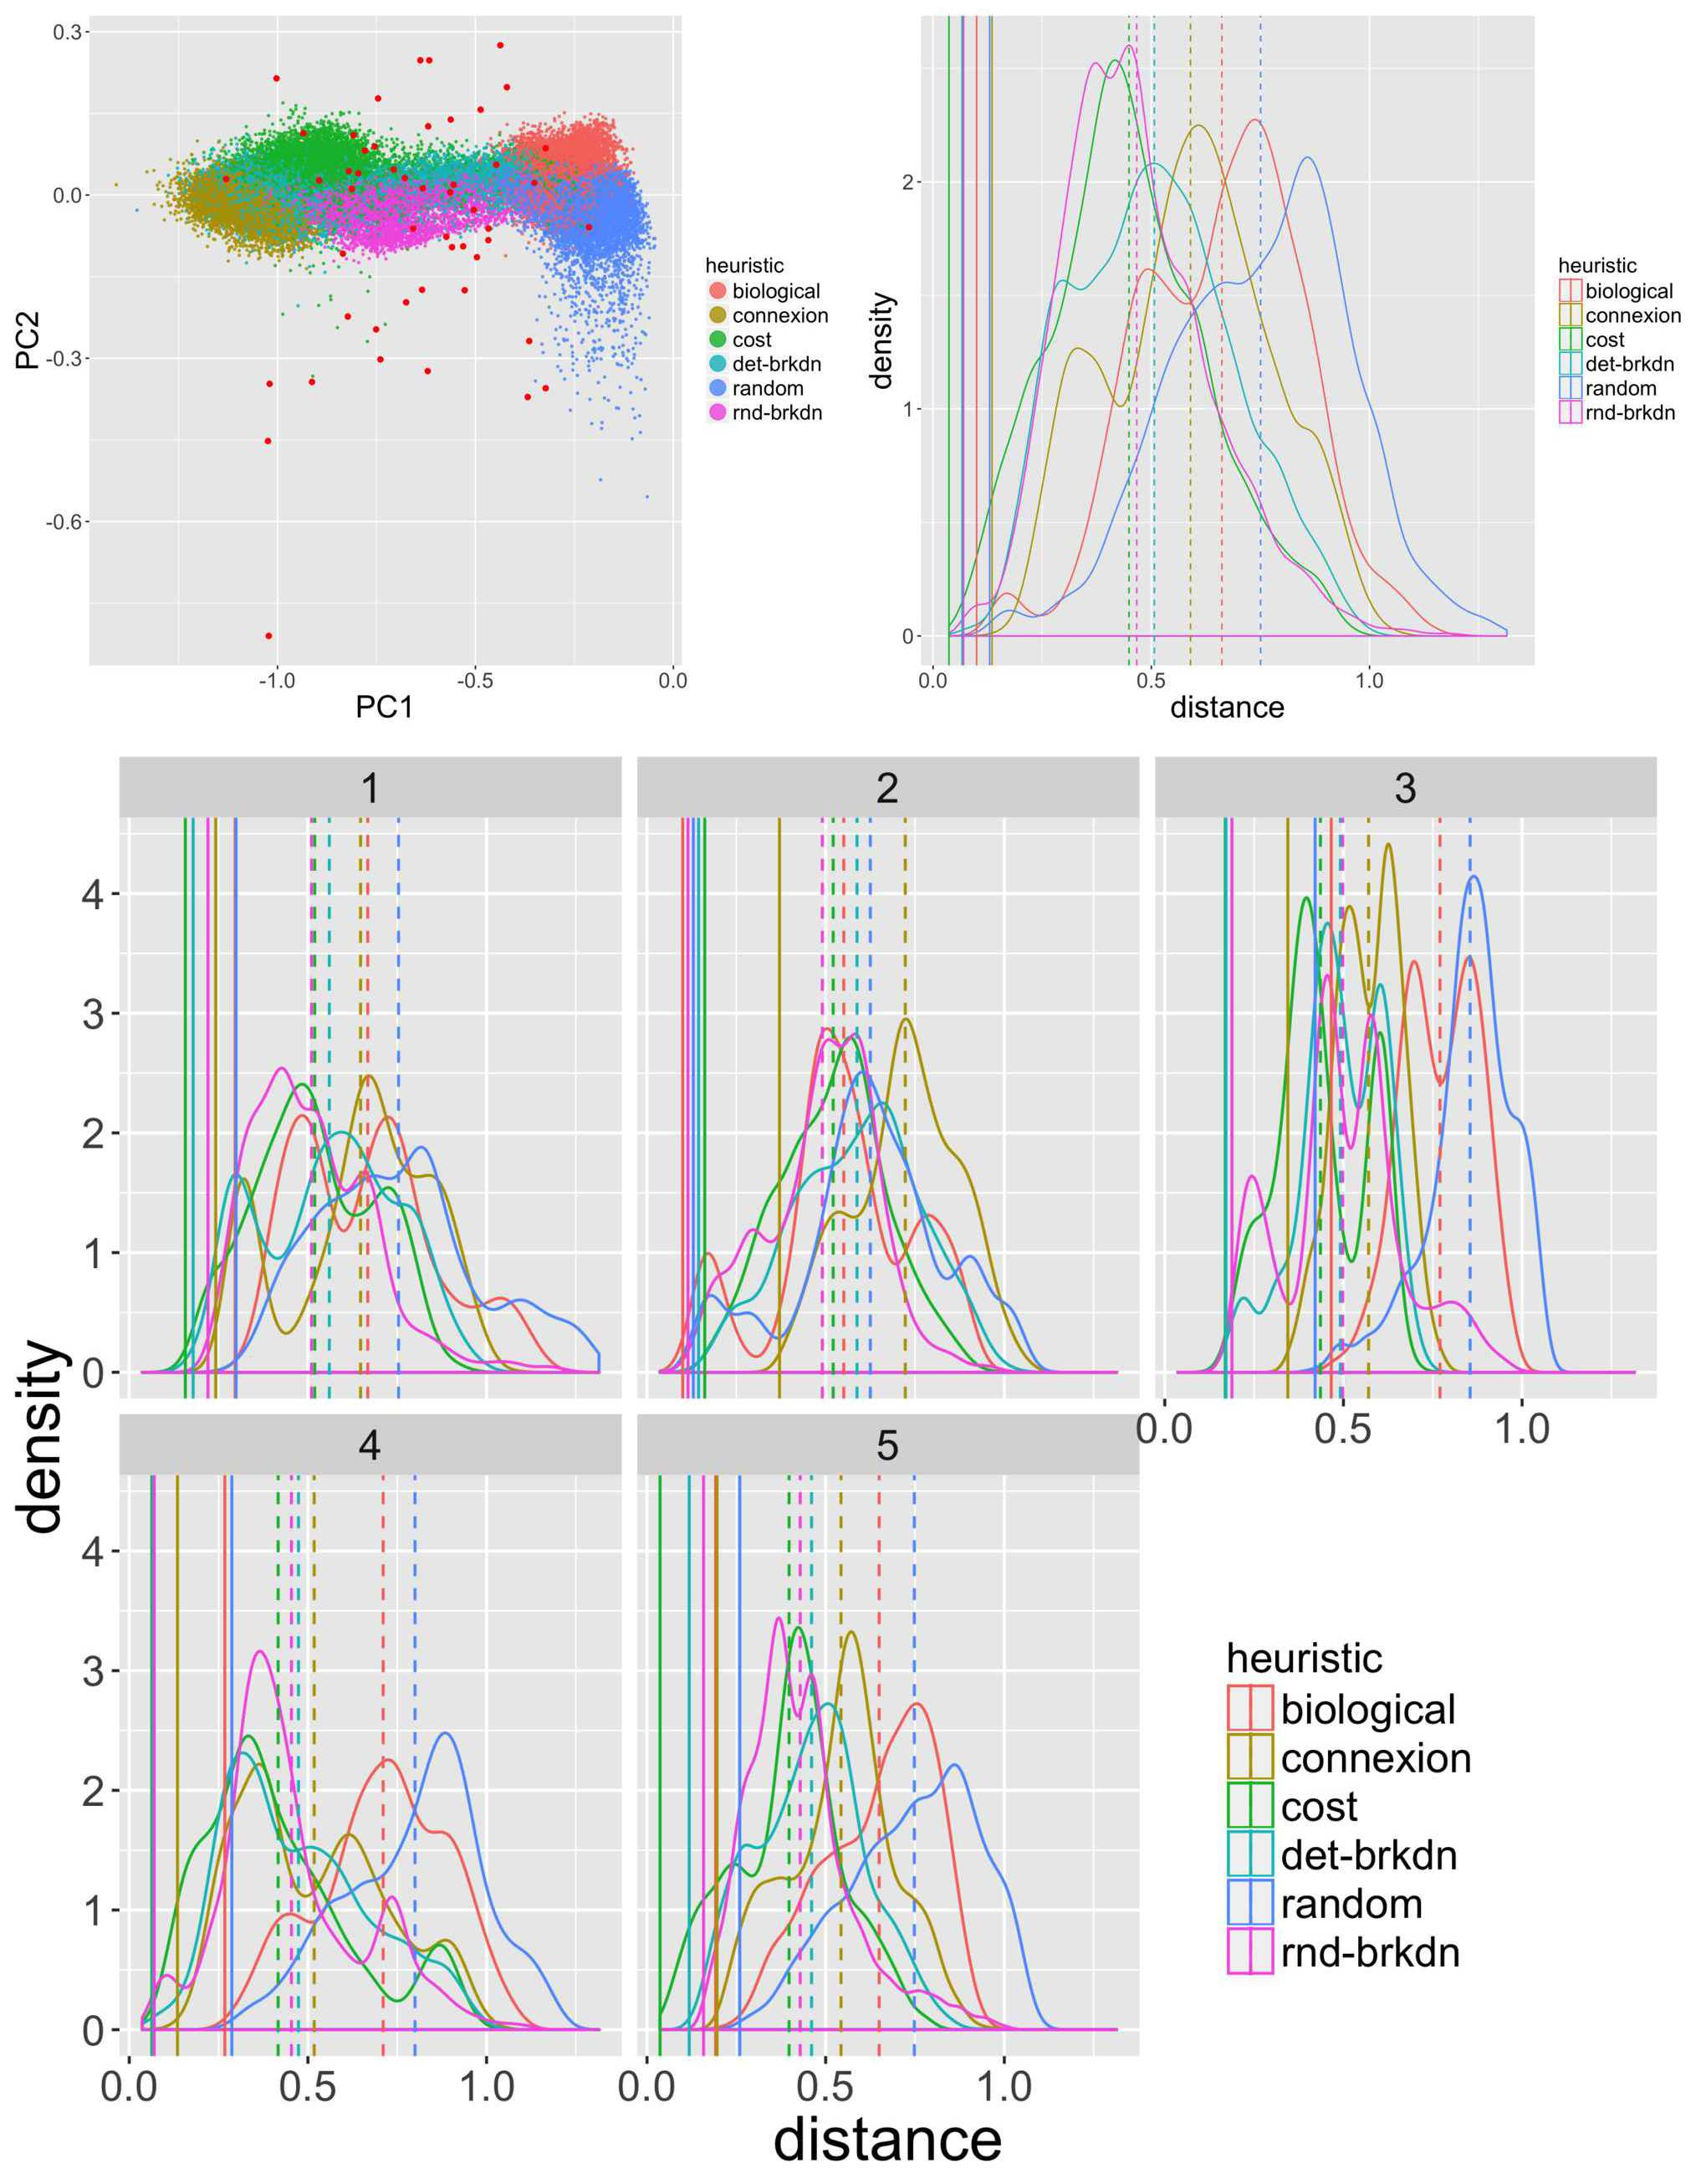
\includegraphics[height=0.8\textheight]{figures/7-1-2-fig-networkgrowth-realdistance.jpg}

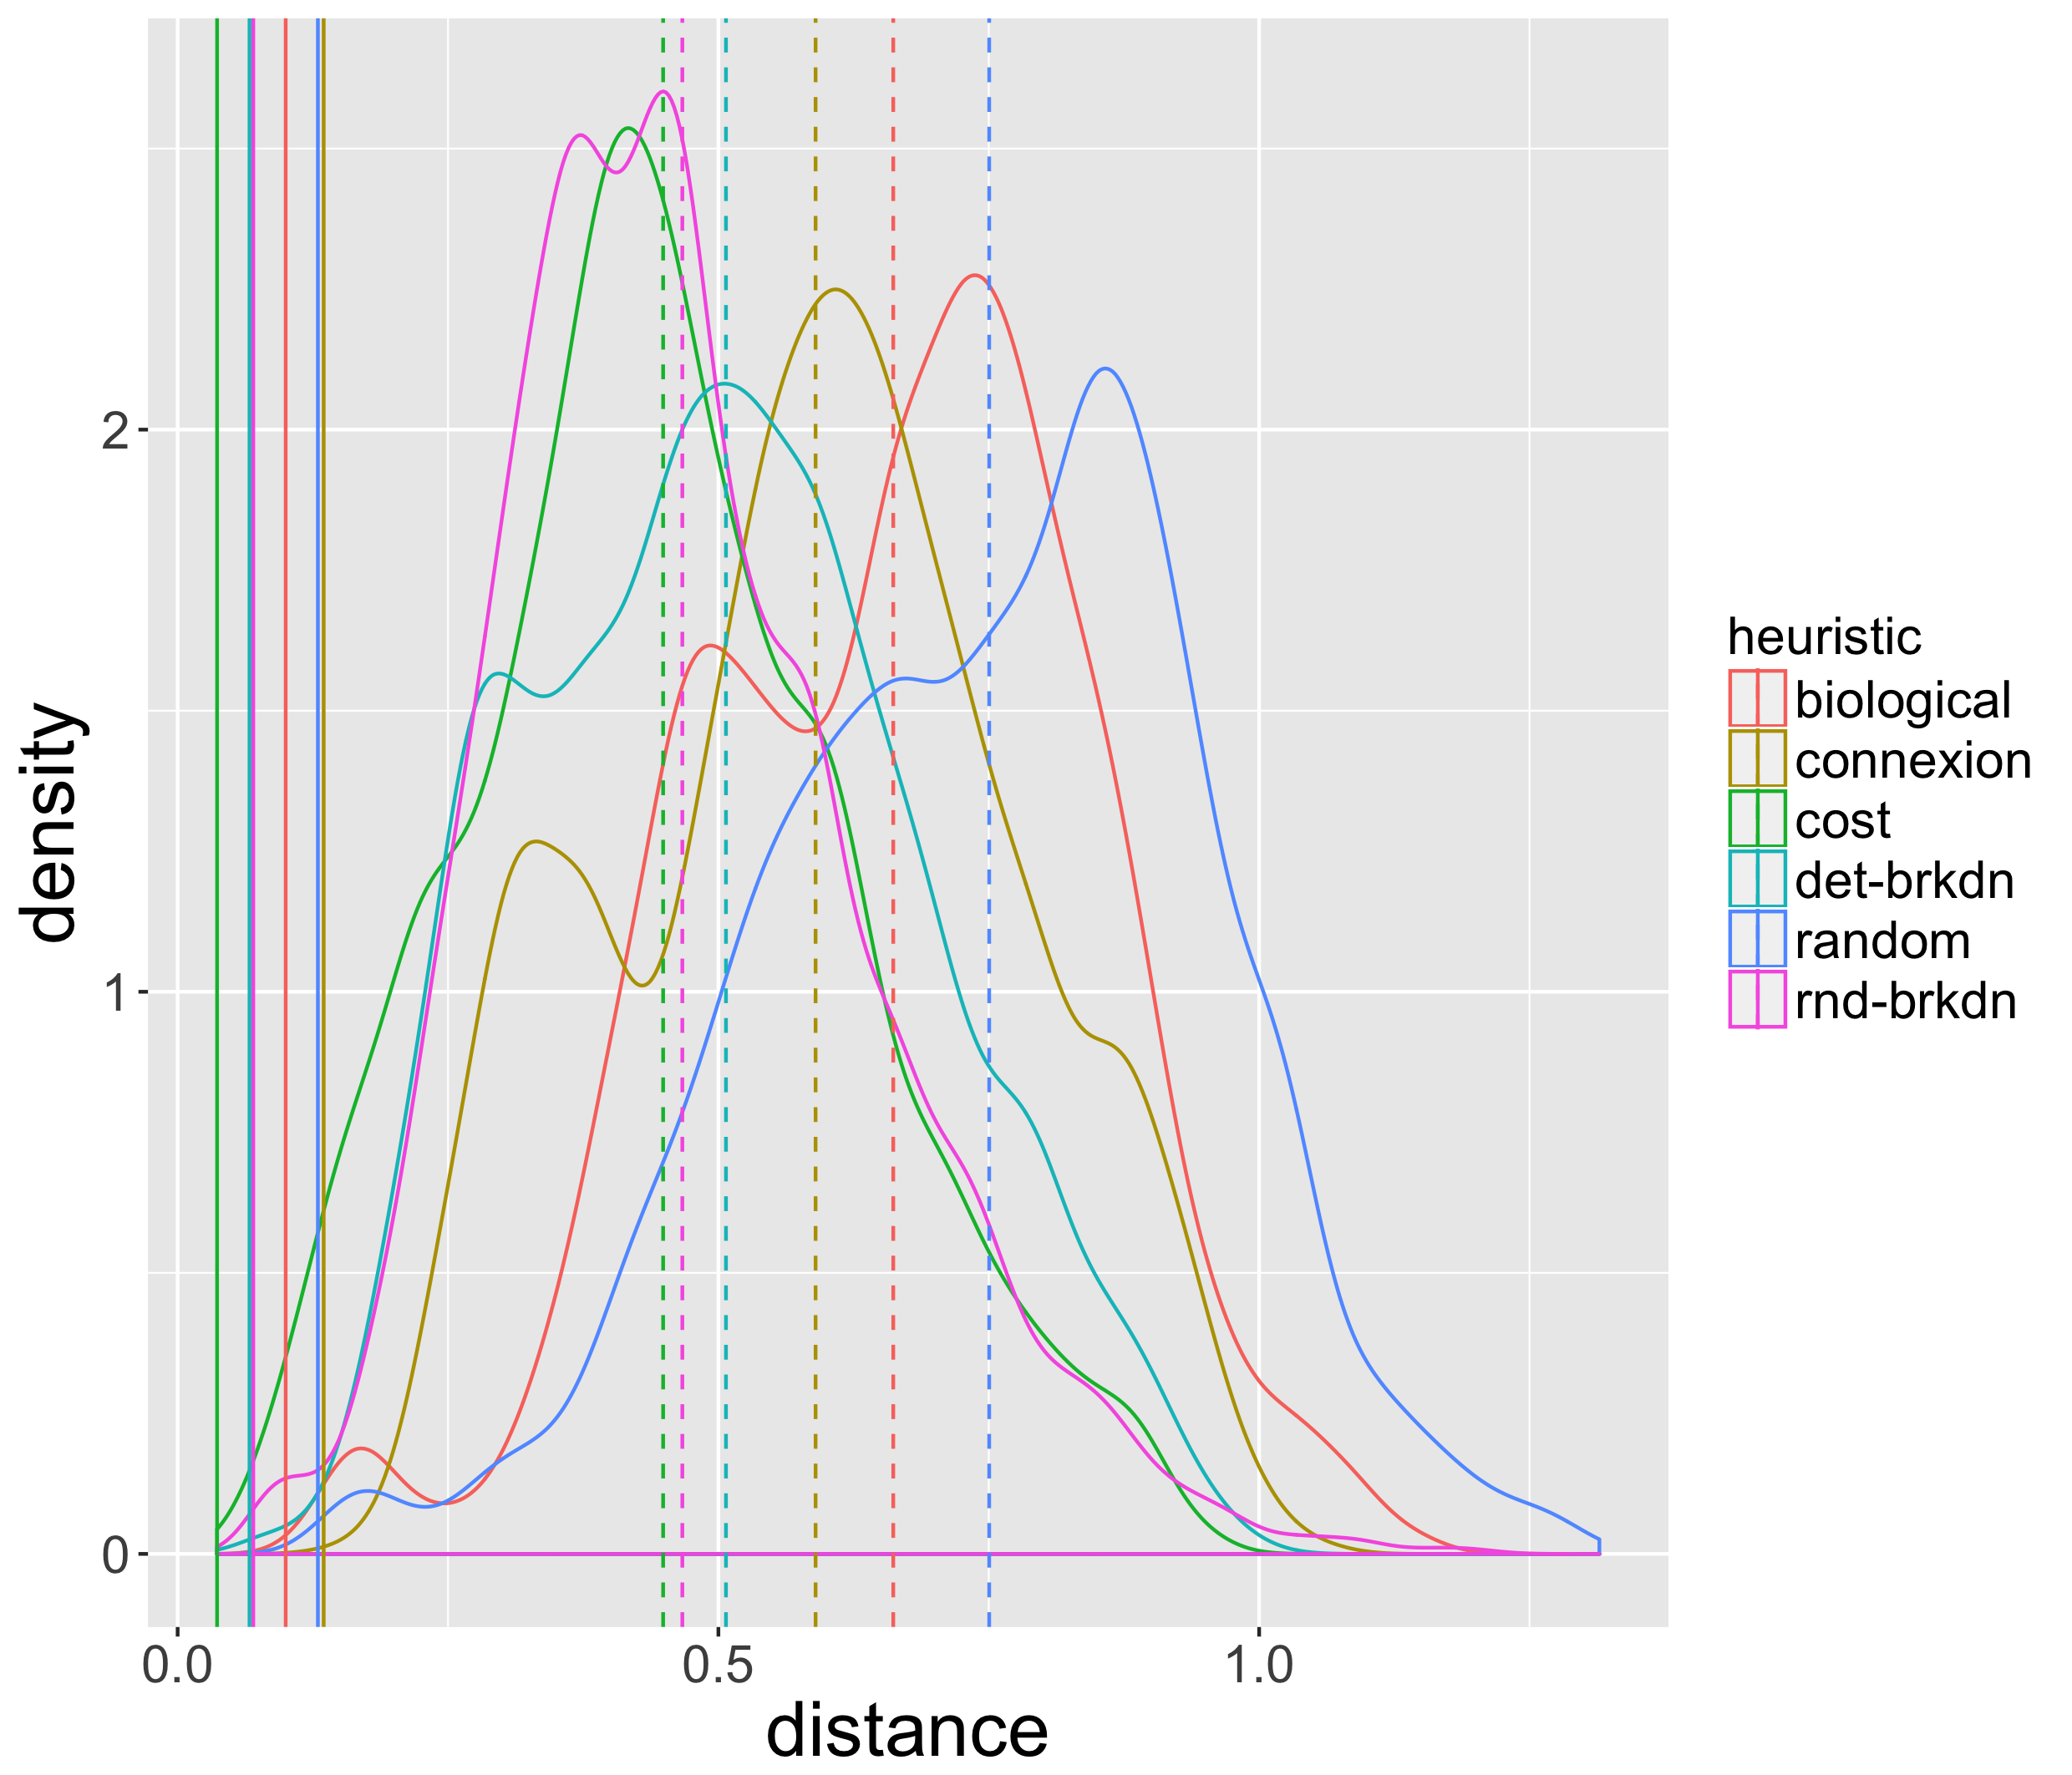
\includegraphics[height=0.8\textheight]{figures/distance_real.png}

\footnotesize \textit{Distribution of distances to topologies of real networks}

}

\sframe{Distance to real networks by density morphology}{

\centering

%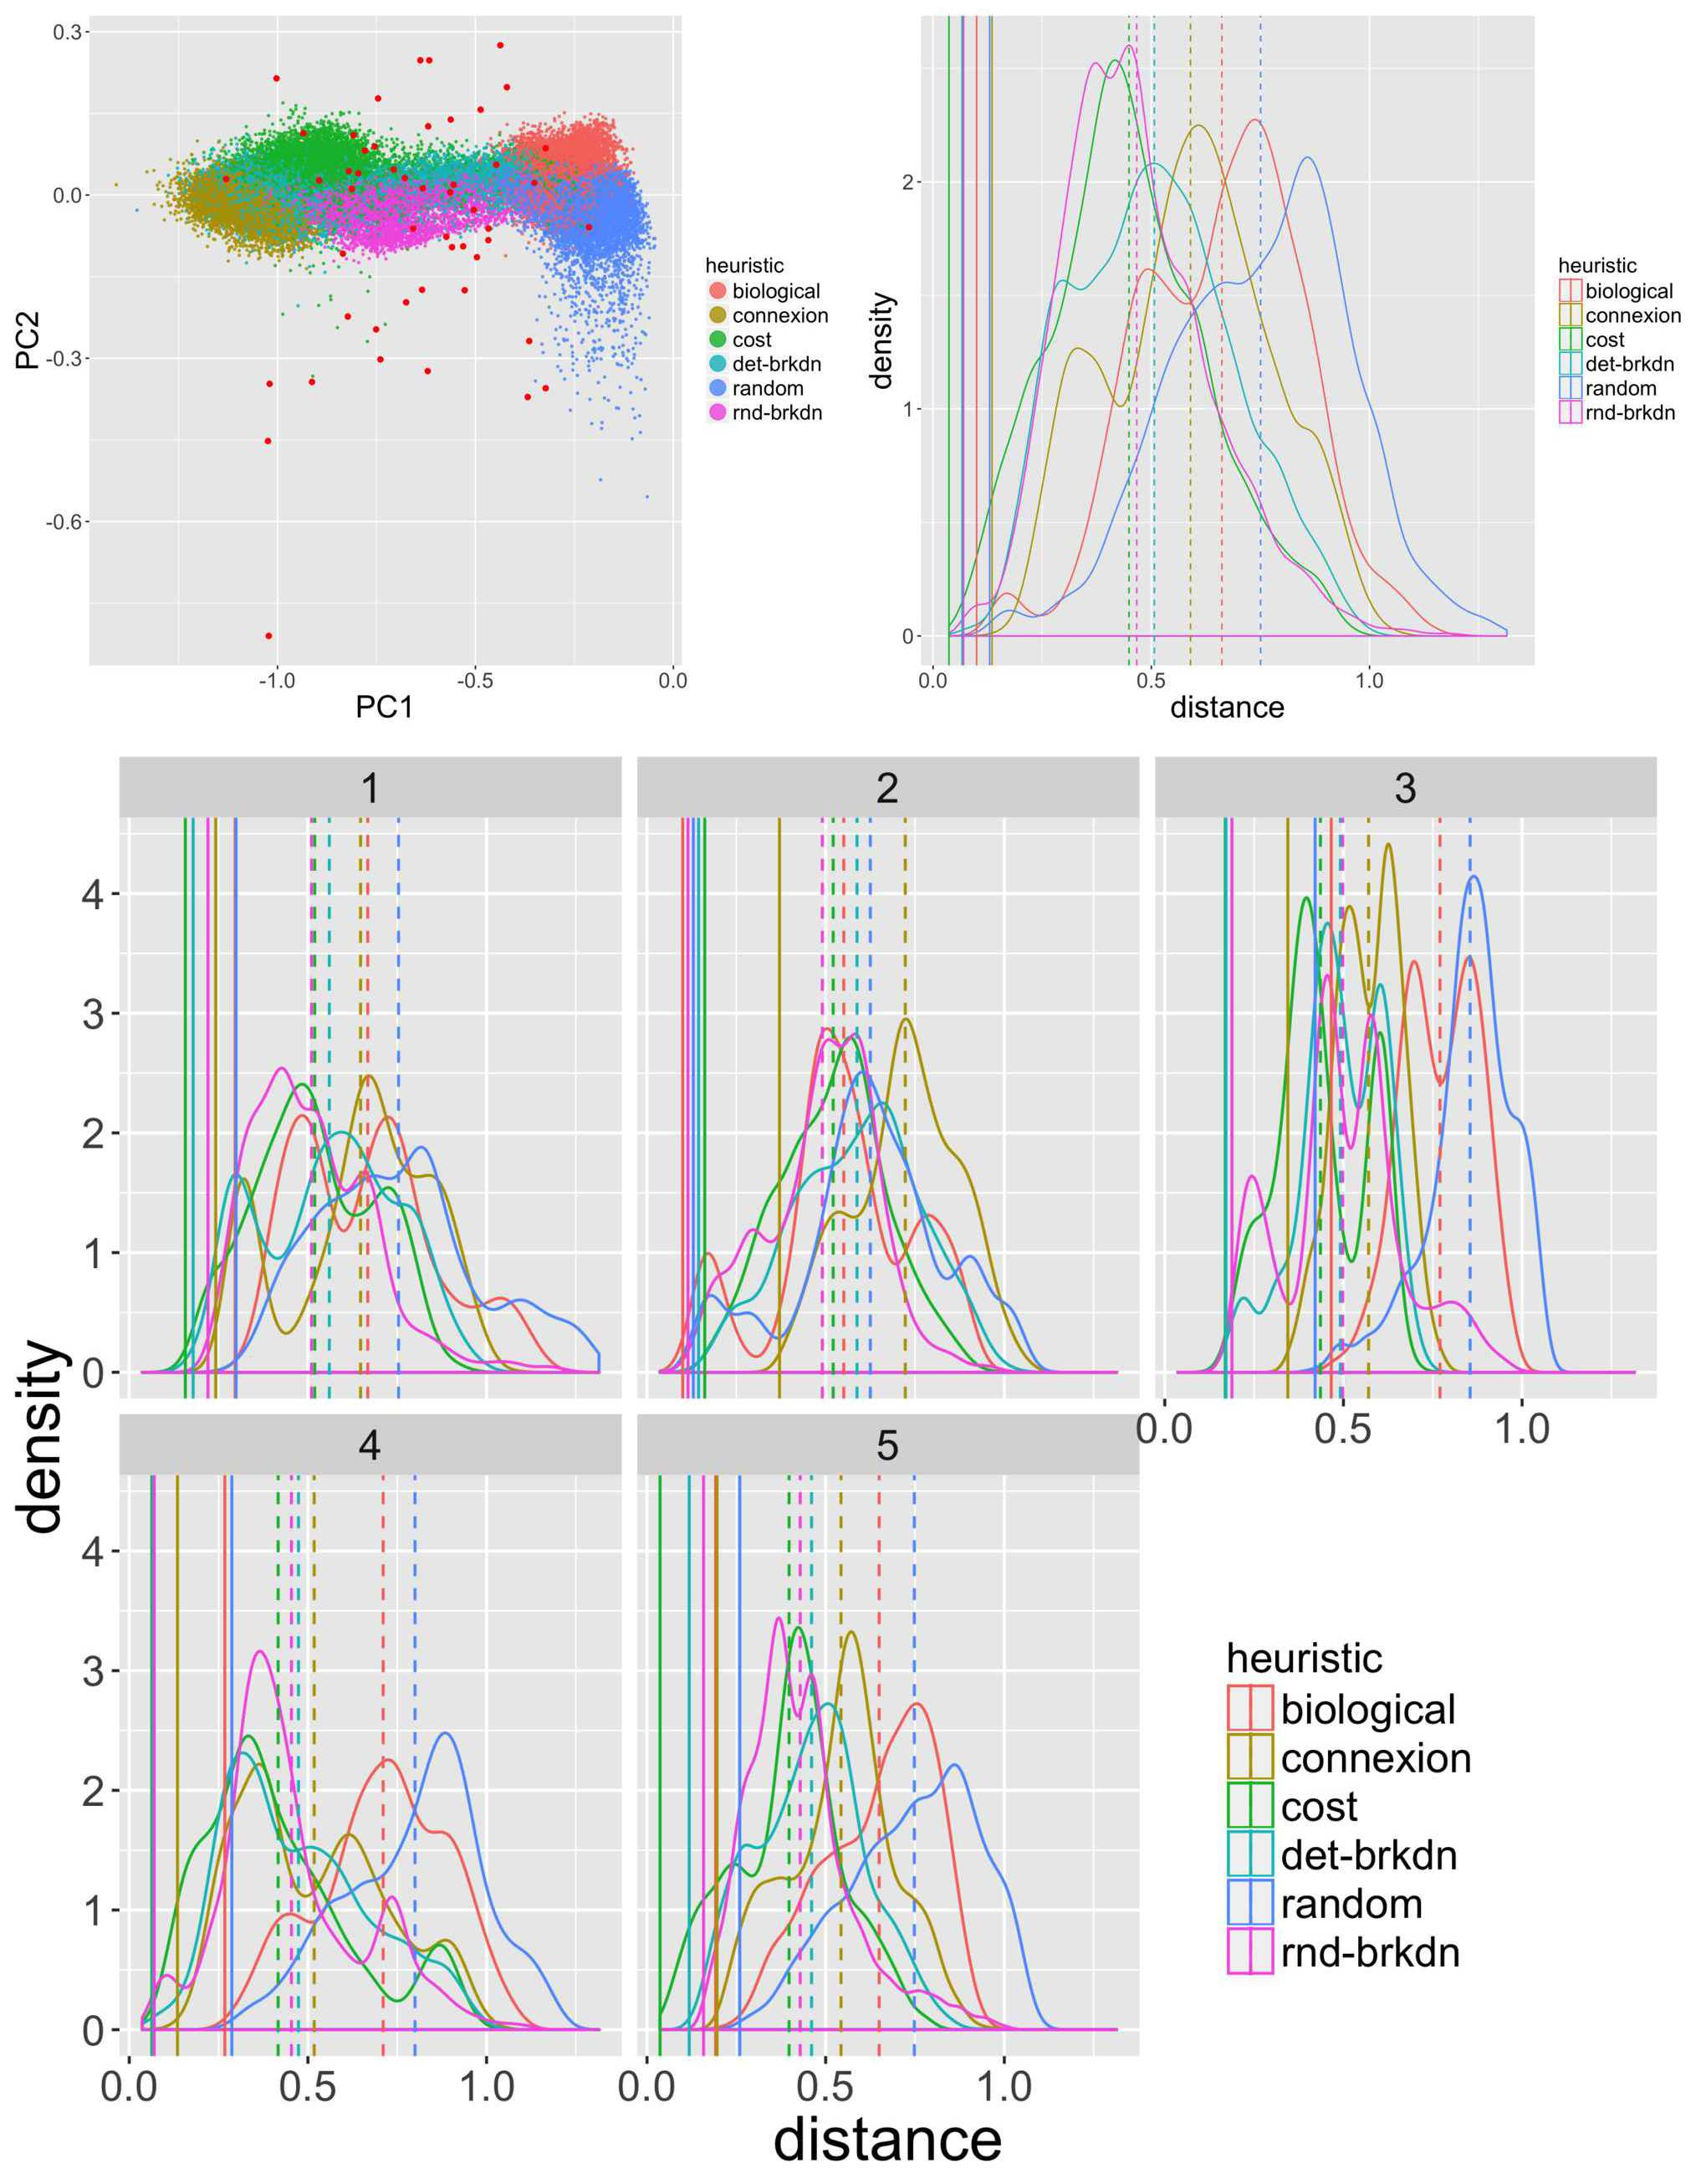
\includegraphics[height=0.8\textheight]{figures/7-1-2-fig-networkgrowth-realdistance.jpg}

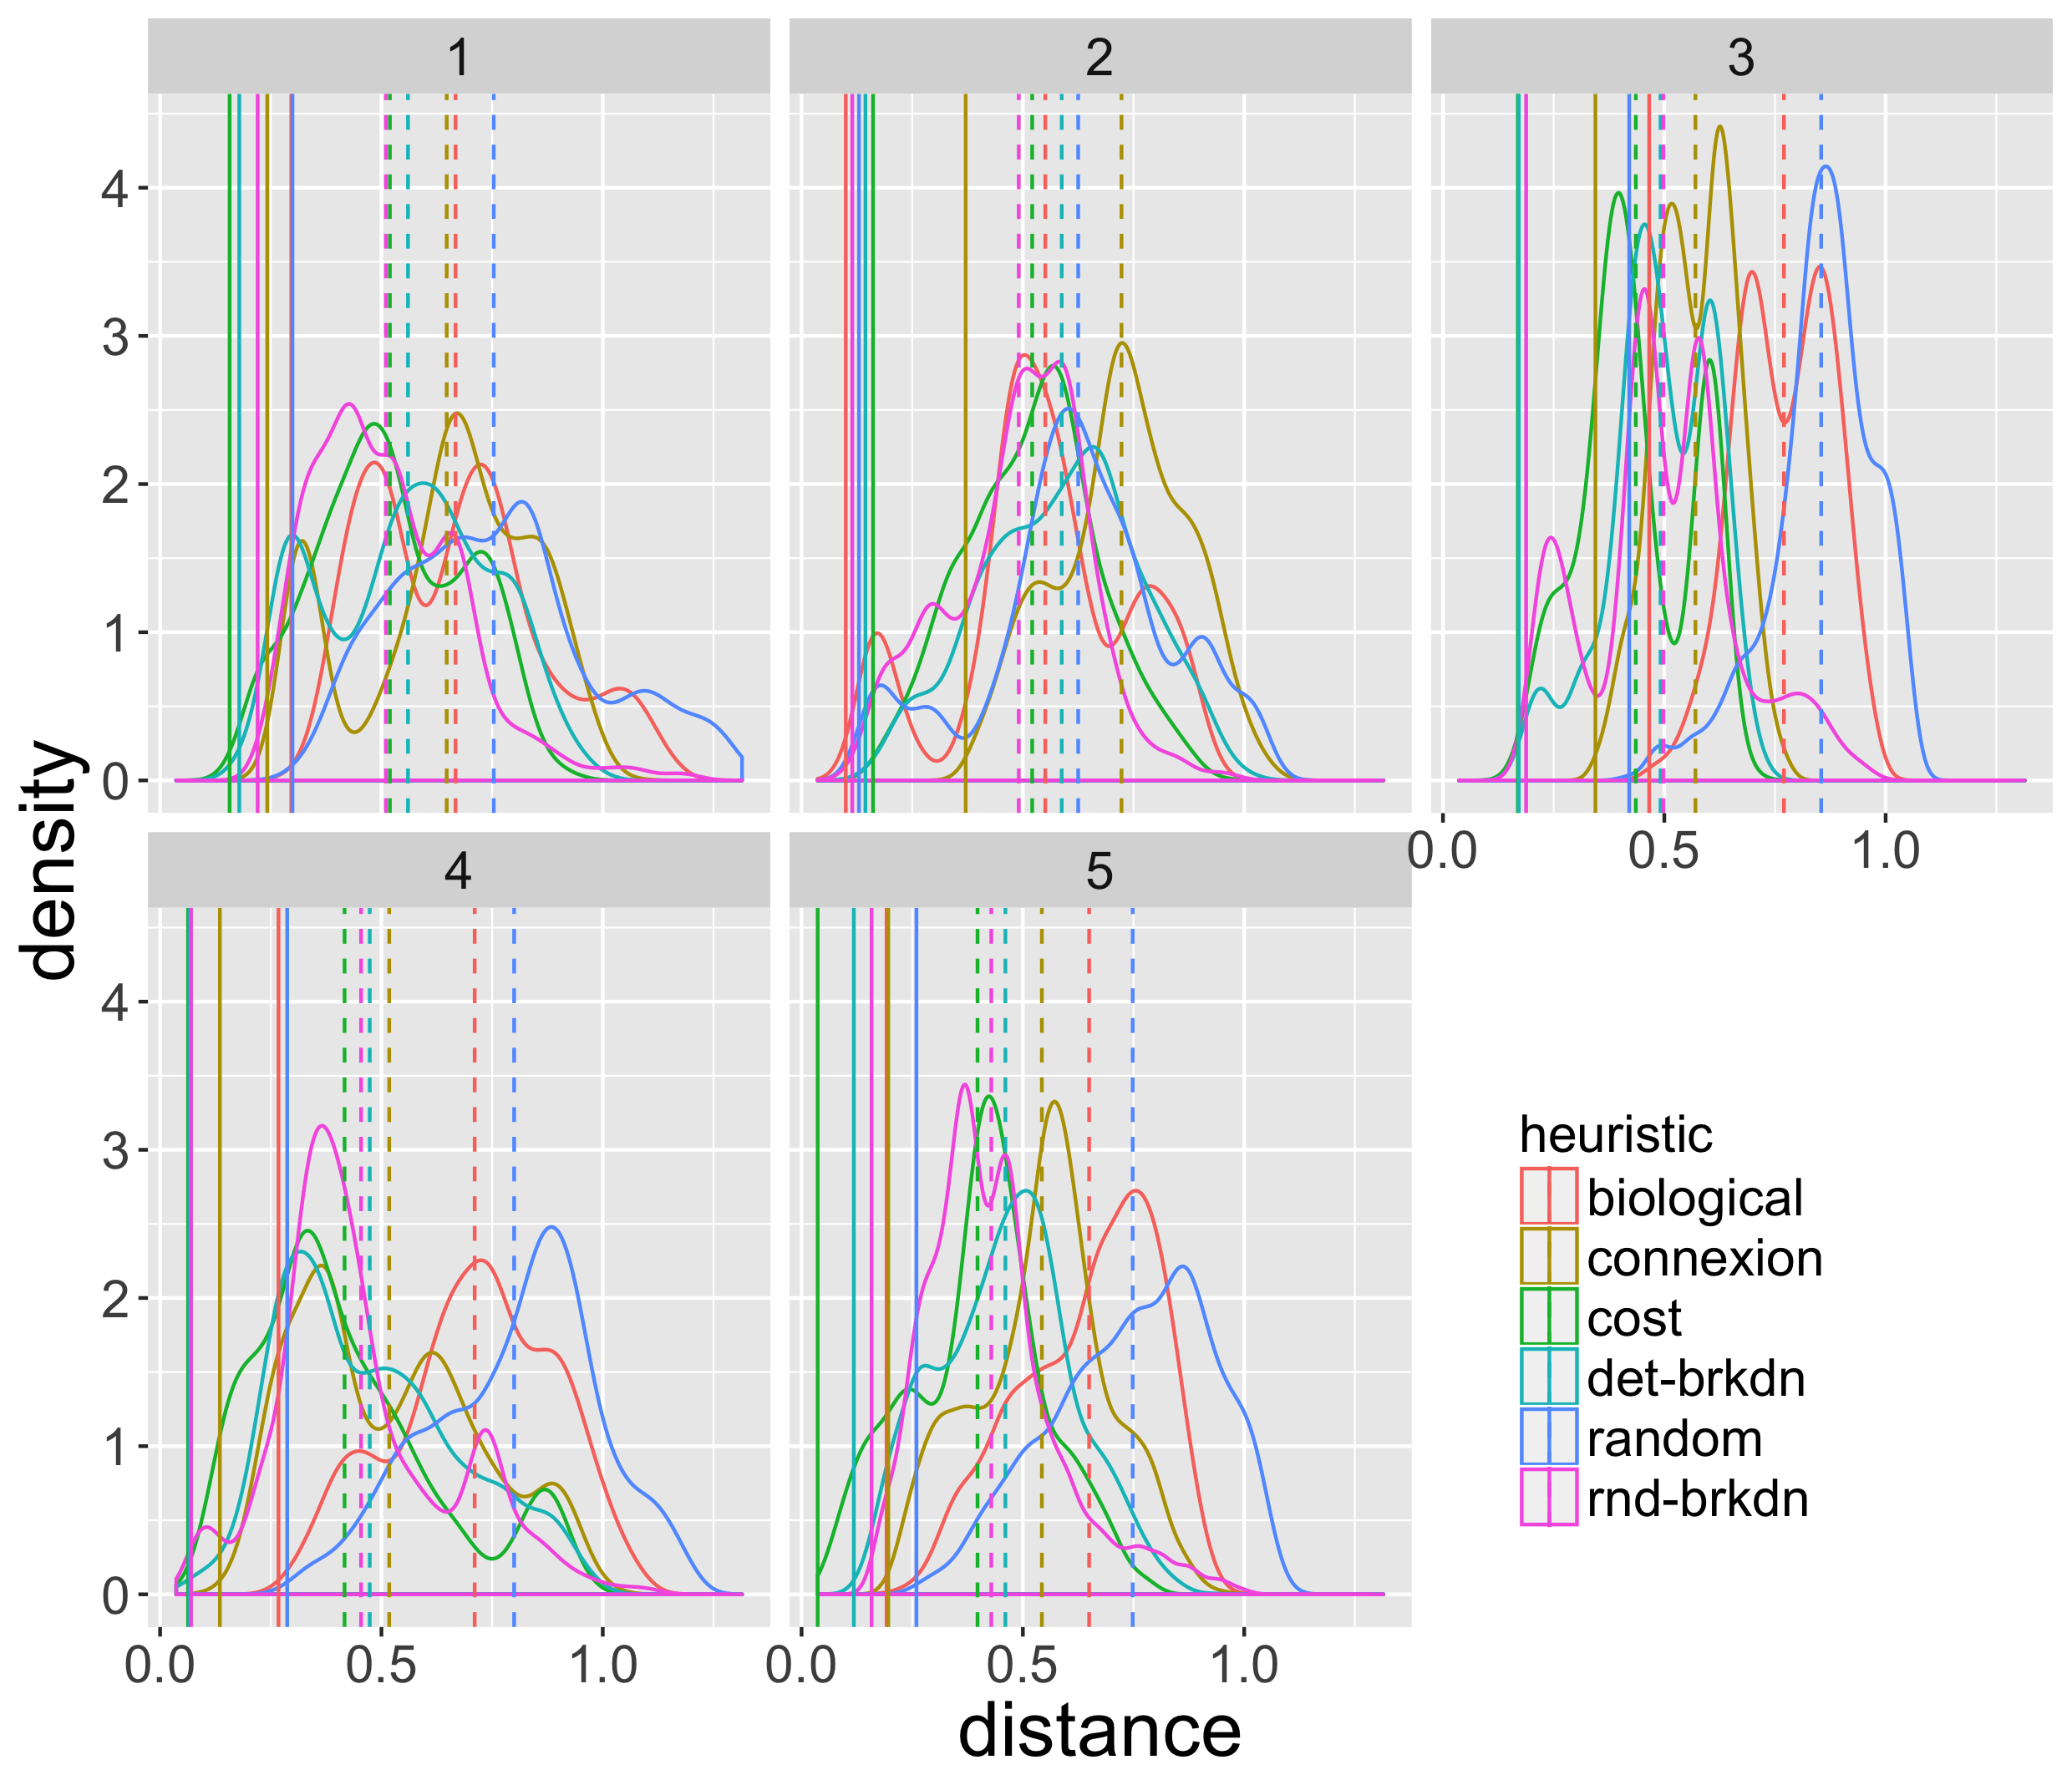
\includegraphics[height=0.8\textheight]{figures/distance_real_bymorph.png}

\footnotesize \textit{Distribution of distances to topologies of real networks, conditioned by classes of population density morphology}

}









% Therefore, our work demonstrates that, among the heuris- tic we compared, there is no best model to reproduce real configurations and that all processes included are comple- mentary.




\sframe{Discussion}{

\justify

\vspace{-1cm}

\textbf{Implications}

$\rightarrow$ Simple processes sufficient to produce reasonable networks: evidence for morphogenesis ? % implications for morphogenesis ?

\smallskip

$\rightarrow$ Complementary of various processes to cover the feasible space and produce existing topologies.





\bigskip

% Possible developments include a more refined cali- bration to find for typical configurations of real networks the heuristic and parameters producing the closest networks, or a comparison between heuristics controlling for the number of parameters to take overfitting into account (which could be here at the origin of the low performance of the biologi- cal heuristic e.g.). We also suggest that similar benchmarks should be more systematically performed for the modeling of complex territorial systems.


\textbf{Developments}


$\rightarrow$ Dynamical calibration requires (quasi-inexistent) data.

\smallskip

$\rightarrow$ Targeted calibrations to establish potential correspondances between processes and network topology.

\smallskip

$\rightarrow$ Compare network generation heuristics in a ``fair'' way (correcting for additional parameters, open question for models of simulation).


}



\sframe{Conclusion}{


\justify

\vspace{-1cm}

$\rightarrow$ Several road network morphogenesis processes explored: \textbf{need for more coupling and comparison of models.}

\medskip

$\rightarrow$ With more refined urban characteristics and other dimensions ? \textbf{Need for more interdisciplinarity.}

\bigskip

\footnotesize

\textbf{Related works}

Raimbault, J., Banos, A., \& Doursat, R. (2014). A hybrid network/grid model of urban morphogenesis and optimization. Proceedings of 4th ICCSA 2014. arXiv:1612.08552.

\medskip	

Raimbault, J. (2017). Calibration of a Density-based Model of Urban Morphogenesis. arXiv preprint arXiv:1708.06743.

\medskip

Raimbault, J. (2018). An Urban Morphogenesis Model Capturing Interactions between Networks and Territories. arXiv preprint arXiv:1805.05195.

\medskip

\textbf{Open repository} (code, data and results) at\\\texttt{https://github.com/JusteRaimbault/CityNetwork}\\\medskip
\textbf{Acknowledgments} : I thank the \textit{European Grid Infrastructure} and its \textit{National Grid Initiatives} (\textit{France-Grilles} in particular) to give the technical support and the infrastructure.


}






\sframe{Reserve slides}{

\centering

\Large

\textbf{Reserve Slides}

}



%%%%%%%%%%
%% Morphogenesis



\sframe{Model parameters}{

\centering

\vspace{-0.2cm}
\begin{tabular}{|p{1.5cm}|c|c|c|c|c|}
  \hline
Heuristic & Param. & Name & Process & Domain & Default\\
  \hline
\multirow{5}{*}{Base}& $l_m$ & added links & growth & $[0;100]$ & $10$ \\\cline{2-6}
 & $d_G$ & gravity distance & potential & $]0;5000]$ & $500$ \\\cline{2-6}
 & $d_0$ & gravity shape & potential & $]0;10]$ & $2$ \\\cline{2-6}
 & $k_h$ & gravity weight & potential & $[0;1]$ & $0.5$ \\\cline{2-6}
 & $\gamma_G$ & gravity hierarchy & potential & $[0.1;4]$ & $1.5$ \\\hline
\multirow{2}{*}{Random}& $\gamma_R$ & random selection  & hierarchy & $[0.1;4]$ & $1.5$ \\\cline{2-6}
& $\theta_R$ & random threshold & breakdown & $[1;5]$ & $2$ \\\hline
Cost-benefits & $\lambda$ & compromise & compromise & $[0;0.1]$ & $0.05$ \\\hline
\multirow{2}{*}{Biological}& $n_b$ & iterations & convergence & $[40;100]$ & $50$ \\\cline{2-6}
& $\theta_b$ & biological th.& threshold & $[0.1;1.0]$ & $0.5$ \\\hline
\end{tabular}

}



\sframe{Model setup}{

\textbf{Synthetic setup: } rank-sized monocentric cities, simple connection with bord nodes to avoid bord effects 

\textbf{Real setup: } Population density raster at 500m resolution (European Union, from Eurostat)

\bigskip

\centering
\frame{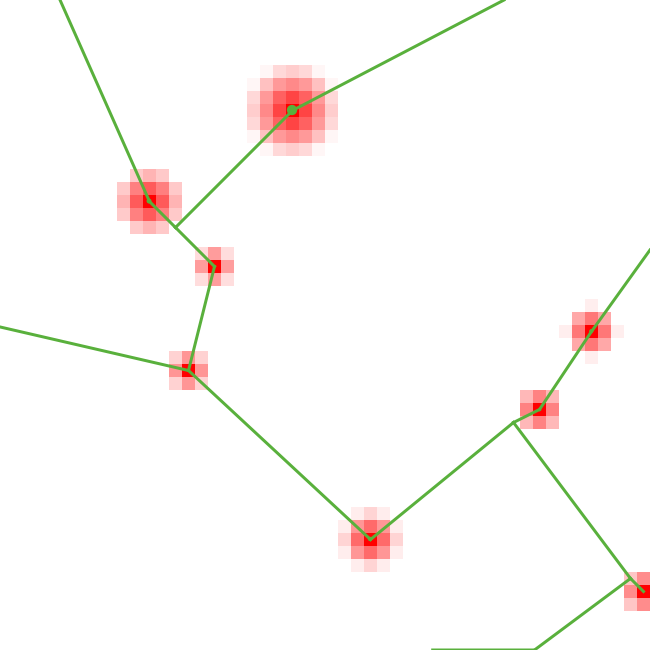
\includegraphics[width=0.35\textwidth]{figures/coevol_example_synthsetup}}\hspace{0.1cm}
\frame{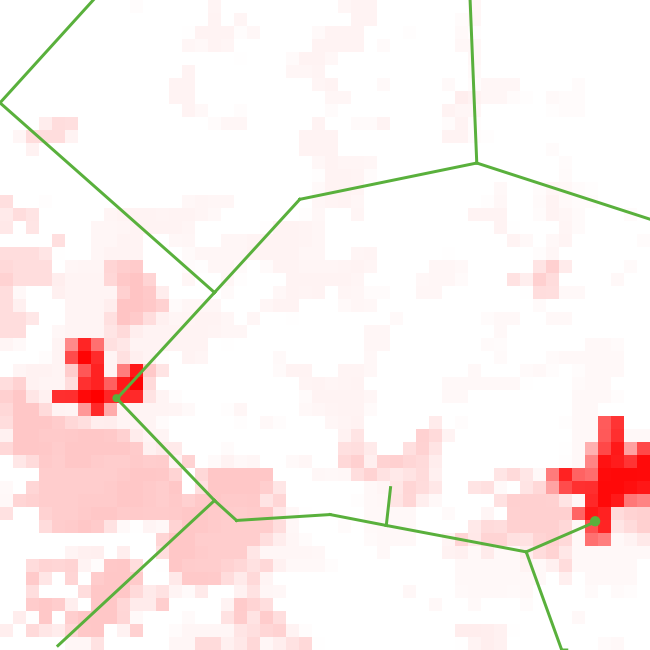
\includegraphics[width=0.35\textwidth]{figures/coevol_example-realsetup}}

\textbf{Stopping conditions: } fixed final time; fixed total population; fixed network size.

}


\sframe{Network Indicators}{

Network Topology measured by:

\begin{itemize}
	\item Betweenness and Closeness centralities: average and hierarchy
	\item Accessibility (weighted closeness)
	\item Efficiency (network pace relative to euclidian distance)
	\item Mean path length, diameter
\end{itemize}

}



\sframe{Network nodes}{

\textbf{Network baseline extension:}

Adding a fixed number $n_N$ of new nodes : for patches such that $d_r < d_0$, probability to receive a node is

% note : not a proba for the last ? no pb as soon as in 0,1, realized anyway.
\[
p = P/P_{max} \cdot (\delta_M - \delta)/\delta_M
\]
% \cdot \exp\left(-((d_r - d_0)/\sigma_r)^2\right)


Nodes connected the shortest way to existing network.

}



\sframe{Biological network morphogenesis model}{

Model studied by~\cite{tero2010rules}: exploration and reinforcement by a slime mould searching for ressources

\medskip

Settings :
\begin{itemize}
	\item Initial homogeneous network of tubes $ij$ of length $L_{ij}$, variable diameter $D_{ij}$, carrying a flow $Q_{ij}$.
	\item Nodes $i$ with a pressure $p_i$.
	\item $N$ nodes are origin/destination points : randomly at each step one becomes source $p_{i_+}=I_0$ and one other sink $p_{i_-}=-I_0$
\end{itemize}


}

\sframe{Biological network evolution}{

At each iteration :
\begin{enumerate}
	\item Determination of flows with Kirchoff's law (electrostatic analogy) : Ohm's law $Q_{ij}=\frac{D_{ij}}{L_{ij}}\cdot(p_{i}-p_{j})$ and conservation of flows $\sum_{j\rightarrow i}Q_{ij} = 0 , \sum_{j\rightarrow i_\pm}Q_{i_{\pm}j} = \pm I_0$
	\item Evolution of diameters ($\gamma$ reinforcement parameter) by
	\[
	\frac{dD_{ij}}{dt}=\frac{\left|Q_{ij}\right|^{\gamma}}{1+\left|Q_{ij}\right|^{\gamma}}-D_{ij}
	\]
\end{enumerate}

\medskip


$\rightarrow$ Extraction of the final network after convergence given a threshold parameter for diameters %(bimodal final distributions)

\medskip

$\rightarrow$ Multi-scale model : diameters are constant during an iteration to obtain equilibrium flows

}



\sframe{Biological network: indicators}{

Behavior of the model evaluated with performance indicators for generated network $(V_f,E_f)$, that are contradictory objectives :
          \bigskip
          \begin{itemize}
          \item Construction costs $c=\sum_{ij\in E_f}D_{ij}(t_f)$
          \bigskip
          \item \begin{justify}Average performance~\cite{banos2012towards}
          \[
          v=\frac{1}{|V_f|^2}\sum_{i,j\in V_f}\frac{d_{i\rightarrow j}}{||\vec{i}-\vec{j}||}
          \]
          \end{justify}
          \bigskip
          \item Robustness (\textit{Network Trip Robustness} index~\cite{sullivan2010identifying})
          \end{itemize}

}


\sframe{Biological network: optimal networks}{

\centering

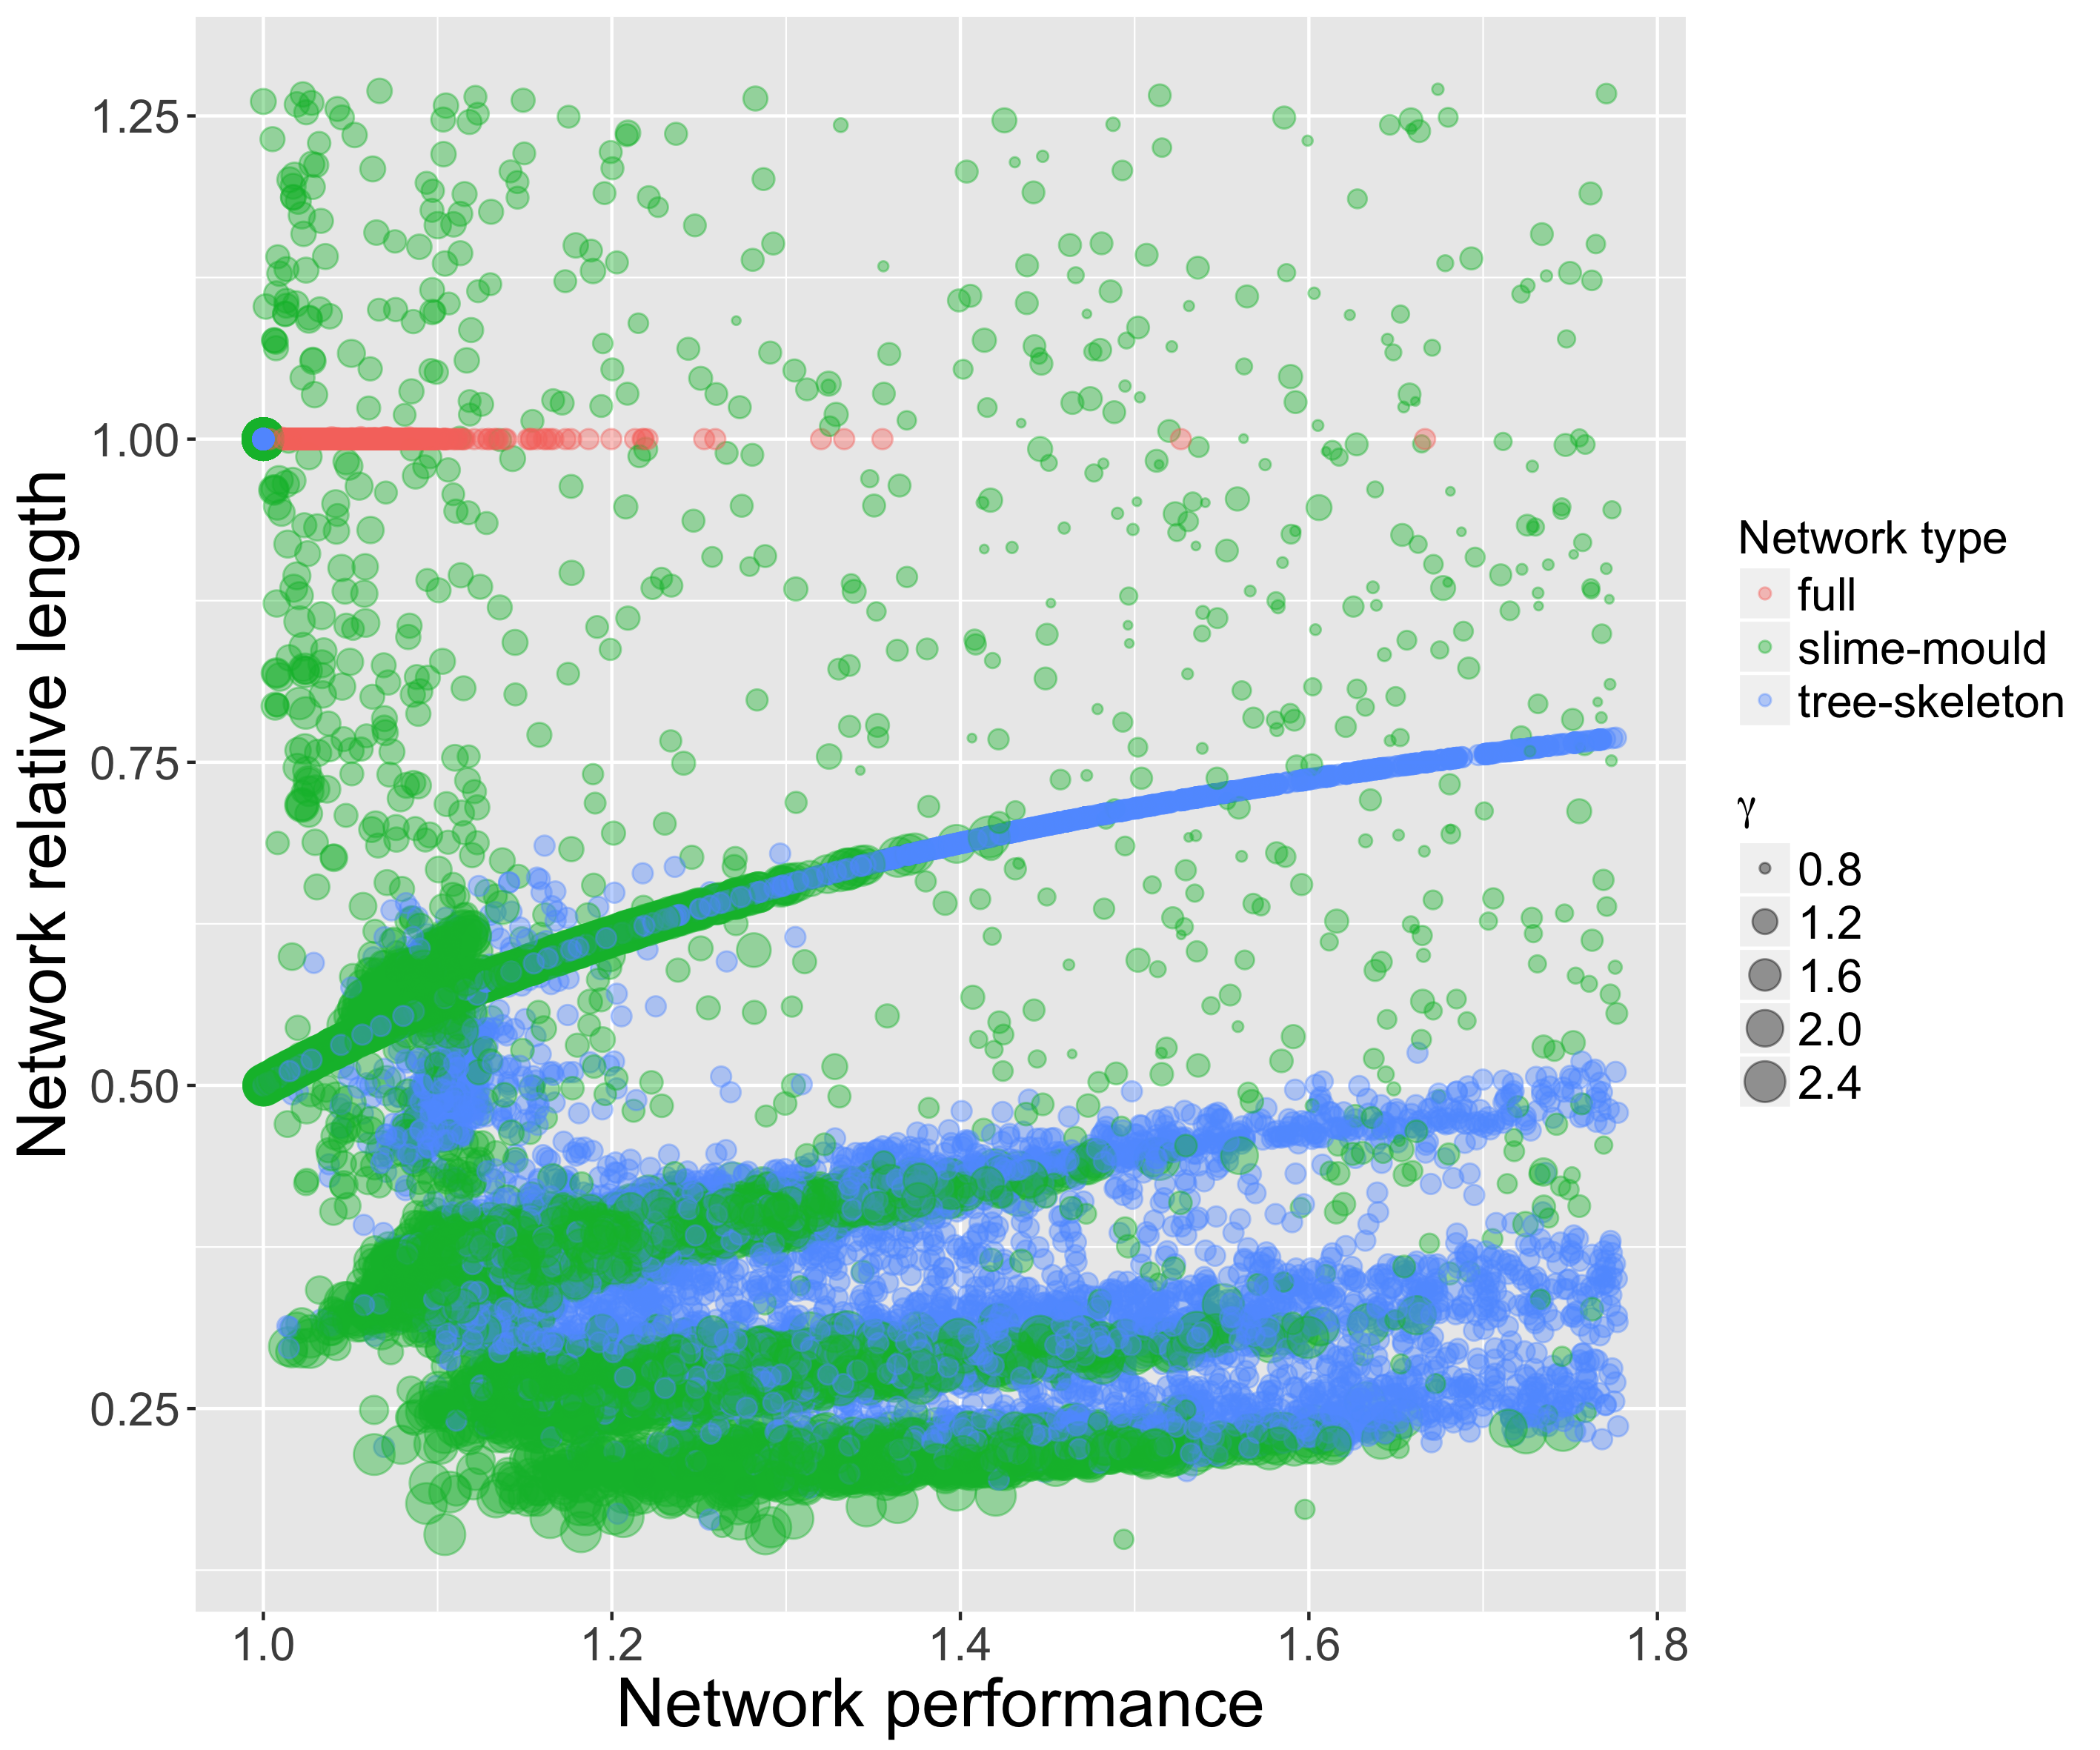
\includegraphics[height=0.8\textheight]{figures/slimemould_paretoSpeedLength.png}

\footnotesize \textit{Exploration of parameter space for synthetic network generation}

}





\sframe{Deterministic breakdown Network generation}{

\begin{enumerate}
\item Gravity potential given by
\[
V_{ij}(d) = \left[ (1 - k_h) + k_h \cdot \left( \frac{P_i P_j}{P^2} \right)^{\gamma} \right]\cdot \exp{\left( -\frac{d}{r_g (1 + d/d_0)} \right)}
\]

\item $k\cdot N_L$ links are selected with lowest $V_{ij}(d_N)/V_{ij}(d_{ij})$, among which $N_L$ links with highest (lest costly) are realized
\item Network is planarized
\end{enumerate}
}





\sframe{Results: components}{

With average betweenness centrality $\bar{bw}$ and average closeness centrality $\bar{cl}$, diameter $r$, average path length $\bar{l}$, relative speed $v_0$

\medskip

\textbf{Simulated point cloud:} $PC1 = - 0.51 \bar{bw} - 0.45 \bar{l} + 0.57 v_0 - 0.43 r + 0.05 \bar{cl}$ and $PC2 = -0.45 \bar{bw} + 0.17 \bar{l} +0.33 v_0 + 0.8 r +0.1 \bar{cl}$

\medskip

\textbf{Herfindhal index} (20 width grid): first quartile at $0.54$, a median at $0.76$ and a third quartile at $1$

\medskip

\textbf{Distance to real configurations:} $d(1,2) = \sqrt{(\bar{bw}_1 - \bar{bw}_2)^2 + (\bar{cl}_1 - \bar{cl}_2)^2 + (\bar{l}_1 - \bar{l}_2)^2}$, we use $d_{min} = \min_j d(S,R_j)$

\medskip

\textbf{Real point cloud:} $PC1 = 0.12 \bar{bw} - 0.09 \bar{cl} + 0.98 \bar{l}$ and $PC2 = -0.20 \bar{bw} - 0.97 \bar{cl} - 0.06 \bar{l}$


}

\sframe{Population morphology classes}{

With 10 grids per class:
\begin{itemize}
	\item Class 5: lowest Moran, high distance, hierarchy and entropy; numerous population centers that are localized and dispersed.
	\item Class 4: highest entropy and hierarchy; a small number of localized centers.
	\item Class 3: lowest distance and entropy; diffuse population.
	\item Class 2: highest Moran; one or a few centers with consequent size.
	\item Class 1: intermediate values for all indicators; a certain number of centers of intermediate size.
\end{itemize}

}


\sframe{Population morphology classes}{

\centering

\begin{tabular}{|c|c|c|c|c|}
\hline
Class & Moran $I$ & Distance $\bar{d}$ & Entropy $\mathcal{E}$ & Hierarchy $\gamma$ \\\hline 
1 & 0.23 & 0.66 & 0.76 & 0.62 \\\hline % medium everything
2 & 0.47 & 0.50 & 0.75 & 0.53 \\\hline % highest moran, medium others
3 & 0.21 & 0.42 & 0.57 & 0.65 \\\hline % lowest distance and entropy, medium slope
4 & 0.24 & 0.75 & 0.90 & 0.87 \\\hline % highest entropy and slope
5 & 0.15 & 0.76 & 0.84 & 0.72 \\\hline % lowest moran, high distance, slope and entropy
\end{tabular}

}





\sframe{What is Morphogenesis ? Examples}{

% illustrations : ants, geomorphology, neurons, self-assembly ; ARBOTRON ; paper nature aile avion
% all from netlogo library ? would be nice illustration of generative nature


% remark : do not put classical biological example to show how it has percolated to other fields

\vspace{-0.3cm}

\includegraphics[width=\textwidth,height=0.82\textheight]{figures/intro_examples}

\justify

\vspace{-0.5cm}

\footnotesize\textit{Sources (in order by column). Ants, Erosion, Game of Life: NetLogo Library ; Arbotron \cite{jun2005formation}; Industrial design \cite{Aage:2017aa}; Swarm chemistry \cite{sayama2009swarm}}
% sources : ants netlogo ; erosion netlogo ; arbotron 
%  inge : 

}



\sframe{What is Morphogenesis ?}{

\textbf{Morphogenesis} (\textit{Oxford dictionary}) 
\begin{enumerate}
\item \textit{Biology} : The origin and development of morphological characteristics
\item \textit{Geology} : The formation of landforms or other structures.
\end{enumerate}

\bigskip

\textbf{History of the notion}

$\rightarrow$ Started significantly with embryology around 1930~\cite{abercrombie1977concepts} 

$\rightarrow$ Turing's 1952 paper~\cite{turing1952chemical}, linked to the development of Cybernetics

$\rightarrow$ first use in 1871, large peak in usage between 1907-1909, increase until 1990, decrease until today. \textit{Scientific fashion ?}


}




\sframe{Interdisciplinary Definition of Morphogenesis}{

% precise notions and defs

\justify

\textit{Construction of an interdisciplinary definition in~\cite{antelope2016interdisciplinary}
}

\bigskip




\textbf{Meta-epistemological framework of imbricated notions:}

Self-organization $\supsetneq$ Morphogenesis $\supsetneq$ Autopoiesis $\supsetneq$ Life


\bigskip

\textbf{Properties:}

\begin{itemize}
\item Architecture links form and function
\item Emergence strength~\cite{bedau2002downward} increases with notion depth, as bifurcations~\cite{thom1974stabilite}
\end{itemize}

\bigskip

\textbf{Definition of Morphogenesis :} \textit{Emergence of the form and the function in a strongly coupled manner, producing an emergent architecture \cite{doursat2012morphogenetic}}



}




\sframe{Modeling Urban Morphogenesis}{

\textit{More or less explicit use of the concept of Morphogenesis in Urban Simulation, depending on the scale and the approach.}

\medskip
                                                                                                                                                                                                                                                                                                                                                                                                                                                                                                                                                                                                        
\begin{itemize}
	\item \cite{makse1998modeling} correlated growth
	\item \cite{10.1371/journal.pone.0133780} multi-scale migration and percolation
	\item \cite{bonin2012modele} qualitative differentiation of urban function
	\item \cite{achibet2014model} procedural model at the micro-scale
	\item \cite{caruso2011morphological} micro-economic model of sprawl
	\item \cite{bonin2014modelisation} urban economics morphogenesis, only work to explicitly mention the morphogen
\end{itemize}


}







\sframe{Extension into a co-evolution model}{

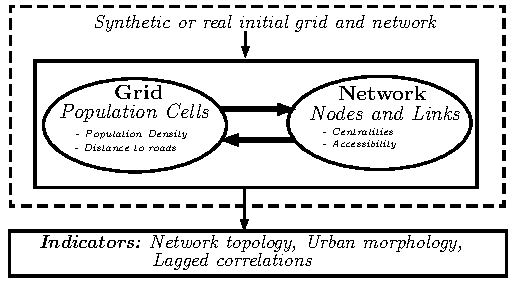
\includegraphics[width=\textwidth]{figures/coevol_mesocoevol}

}




\sframe{Generated Urban Shapes: urban form}{

\centering

\frame{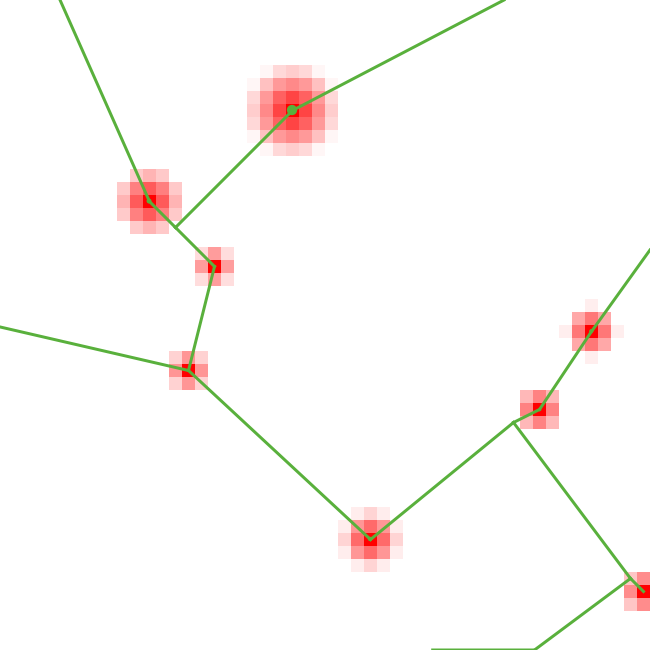
\includegraphics[width=0.28\textwidth]{figures/coevol_example_synthsetup}}\hspace{0.1cm}
\frame{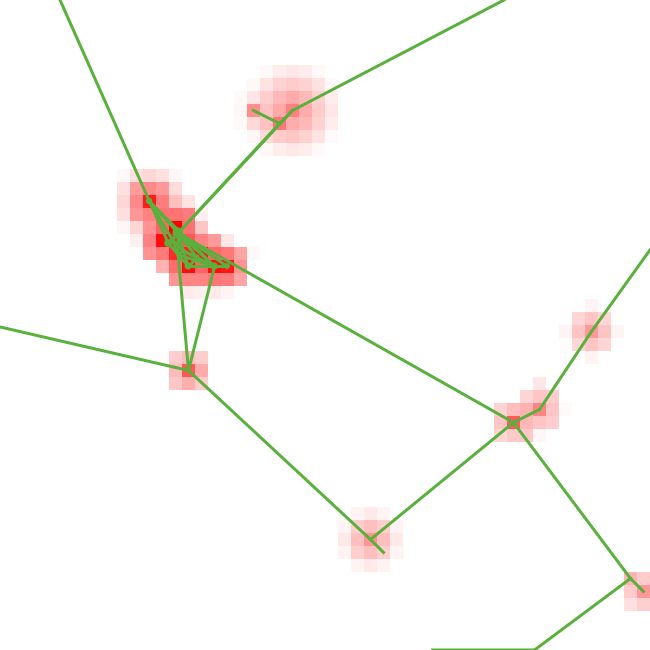
\includegraphics[width=0.28\textwidth]{figures/coevol_example_form-accessonly}}\hspace{0.1cm}
\frame{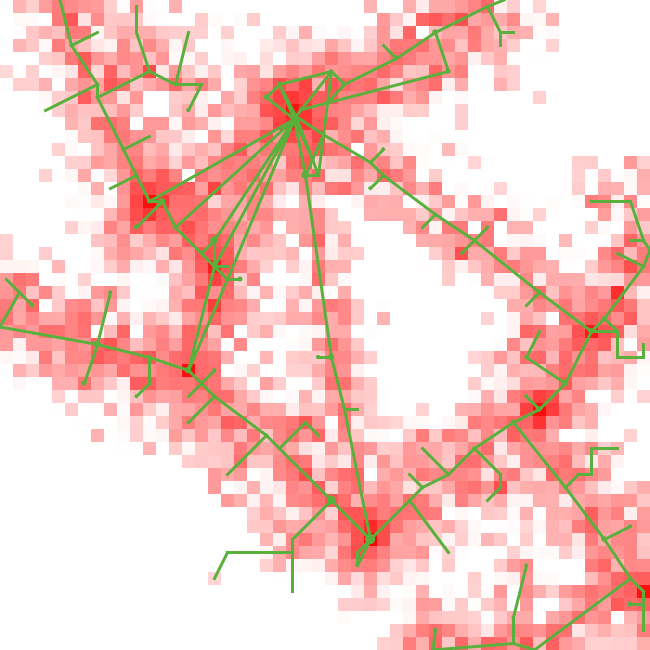
\includegraphics[width=0.28\textwidth]{figures/coevol_example_form-droadonly}}\\\vspace{0.1cm}
\frame{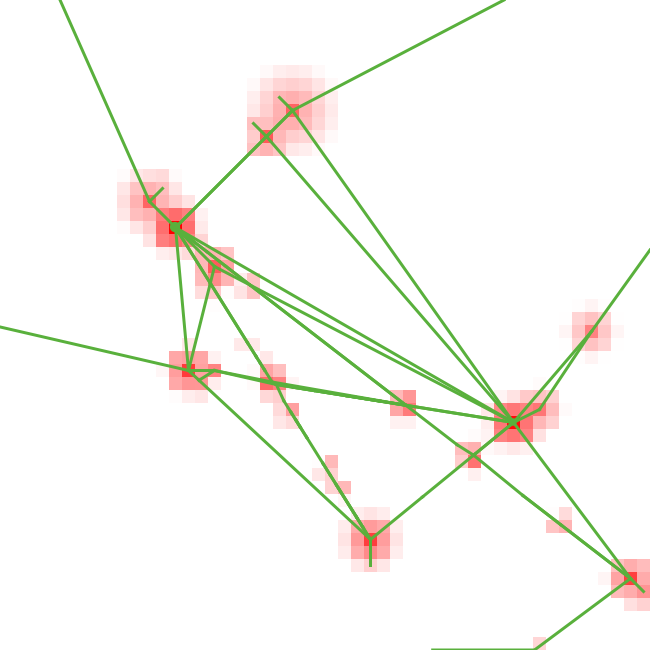
\includegraphics[width=0.28\textwidth]{figures/coevol_example_form-bwonly}}\hspace{0.1cm}
\frame{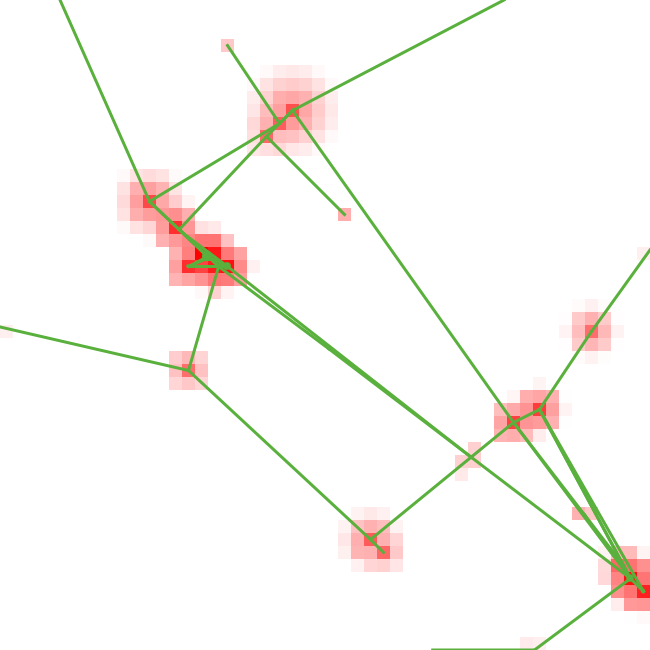
\includegraphics[width=0.28\textwidth]{figures/coevol_example_form-closenessonly}}\hspace{0.1cm}
\frame{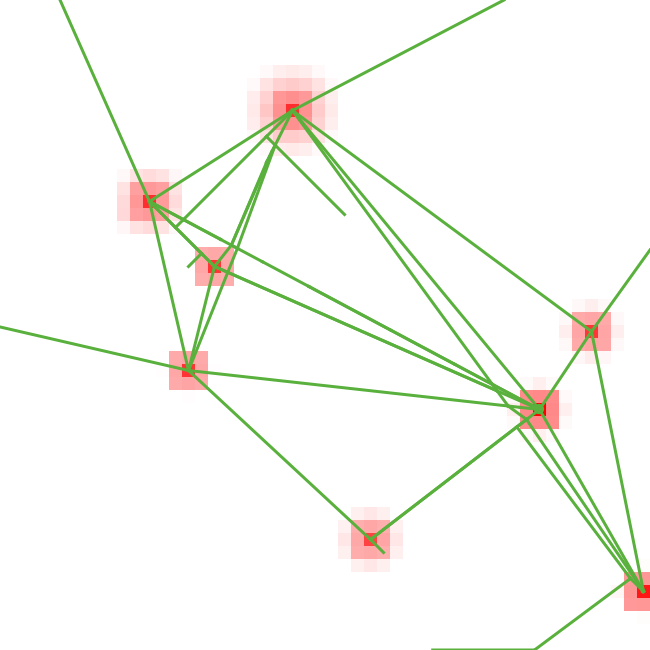
\includegraphics[width=0.28\textwidth]{figures/coevol_example_form-poponly}}

\footnotesize\textit{In order: setup; accessibility driven; road distance driven; betweenness driven; closeness driven; population driven.}

}




%%%%%%%%%%%%%%%%%%%%%
\begin{frame}[allowframebreaks]
\frametitle{References}
\bibliographystyle{apalike}
\bibliography{/Users/juste/ComplexSystems/CityNetwork/Biblio/Bibtex/CityNetwork,biblio}
\end{frame}
%%%%%%%%%%%%%%%%%%%%%%%%%%%%




%\sframe{Example of networks}{
% 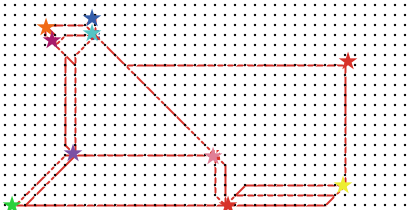
\includegraphics[width=0.48\textwidth]{figures/slimemould_networkDense}
% \hfill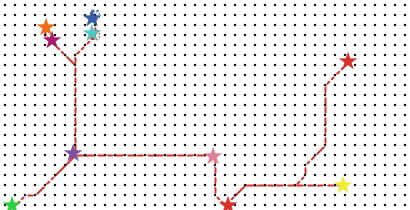
\includegraphics[width=0.48\textwidth]{figures/slimemould_networkLessDense}\\
%          \bigskip
% \justify
%          \textit{Sensitivity of network topology to reinforcement coefficient $\gamma$. Left : $\gamma \sim 1$, robust network. Right : $\gamma >> 1$, arborescent network.}
%}




%\sframe{Sensitivity analysis}{
% 
%          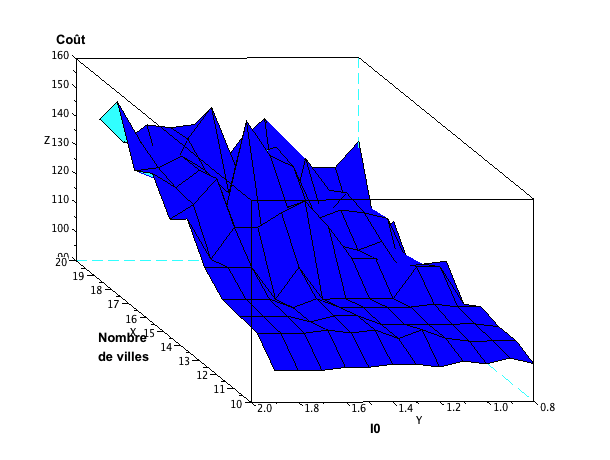
\includegraphics[width=0.5\textwidth]{figures/slimemould_graphe_cout}
%          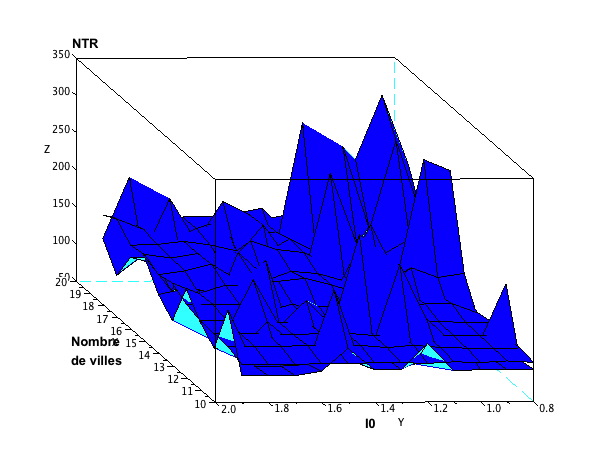
\includegraphics[width=0.5\textwidth]{figures/slimemould_graphe_NTR}\\
%          \bigskip
%          \textit{Sensitivity of indicators to parameters $(N,I_0)$.}
%}




%\sframe{Application : Optimal Network Design}{
%\footnotesize
%$\rightarrow$ Mission of prospective for Romainville city : itinary of an intra-urban shuttle with imposed stops.
%\medskip
%$\rightarrow$ NP-hard problem similar to a Travelling Salesman Problem, but multi-objective (cost, speed, robustness). The bottom-up network generation applied on the initial street network gives a compromise solution.
%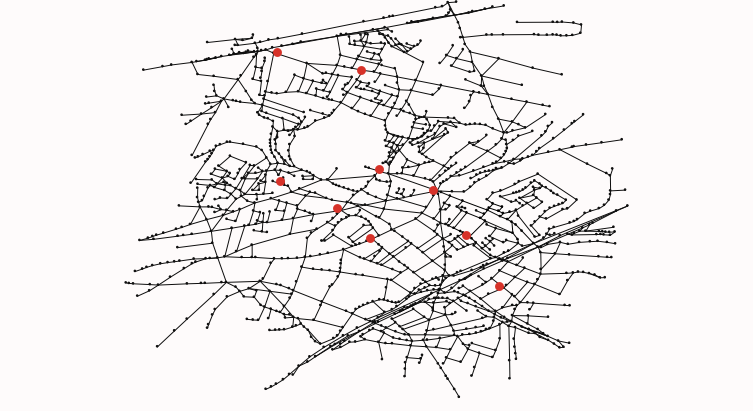
\includegraphics[width=0.32\columnwidth]{figures/slimemould_tick1}
%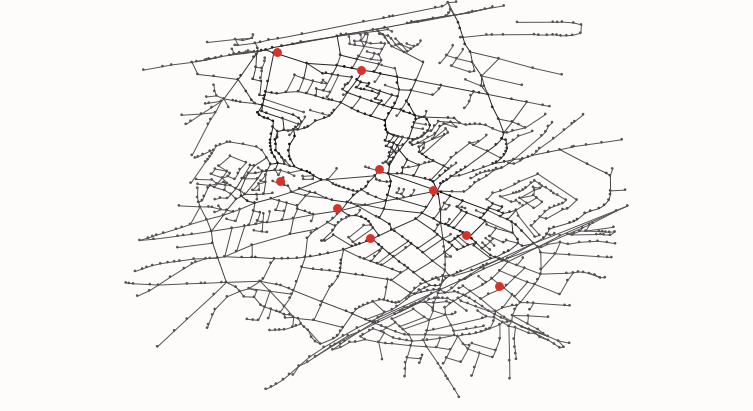
\includegraphics[width=0.32\columnwidth]{figures/slimemould_tick10}
%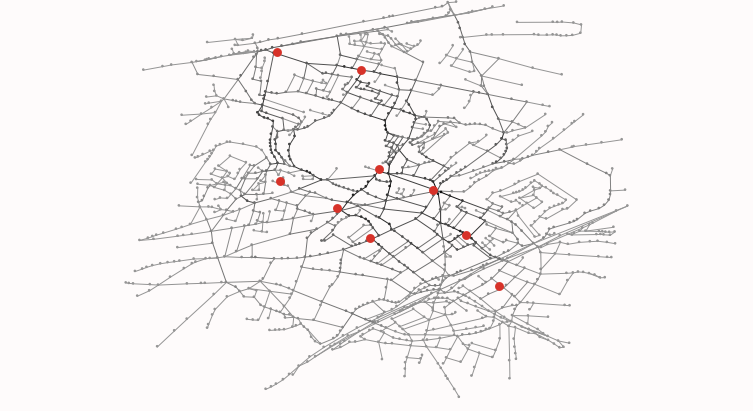
\includegraphics[width=0.32\columnwidth]{figures/slimemould_tick20}\\
%\includegraphics[width=0.32\columnwidth]{figures/slimemould_tick50}
%\includegraphics[width=0.32\columnwidth]{figures/slimemould_tick101}
%\includegraphics[width=0.32\columnwidth]{figures/slimemould_reseauFinal}\\
%\textit{Progressive convergence of the network towards an optimal network connecting the fixed points (in red), starting from the initial street network.}
%}


%\sframe{Application : Optimal transportation Corridor}{   
%Abstract application : \textit{Given a distribution of nodes to serve (sinks), what is the optimal corridor for an infrastructure at a larger scale (train or metro) for which stations are sources, in the sense of the multi-objective optimality of the local self-organized network ?}
%\medskip
%$\rightarrow$ Heuristic exploration of an arborescent set of potential infrastructures
%\medskip
%\includegraphics[width=0.48\textwidth]{figures/slimemould_implantationtree}
%\hfill \includegraphics[width=0.48\textwidth]{figures/slimemould_ImplantationTreeview}      	
%\textit{Heuristic tree to explore infrastructures.}
%\textit{Example of network generation for a given infrastructure.}         
%}         
          
%\sframe{Pareto Optimisation}{
%%\centering
%\includegraphics[width=0.48\textwidth]{figures/slimemould_implantationcntr}
%\includegraphics[width=0.48\textwidth]{figures/slimemould_implantationntrspeed}  
%\textit{Pareto optimisation : projection of explored configurations in indicator space to obtain the Pareto front.}          
%}
%
%\sframe{Pareto Optimisation}{
%\centering
%  \includegraphics[width=0.8\textwidth]{figures/slimemould_paretosimplantation}
%\medskip
%\textit{Configurations corresponding to three optimal points.}
%}





\end{document}









